% get vuw logos from https://wgtn.brandkit.io/assets?tags=National%0Identity
\documentclass{beamer}
%\usepackage[utf8]{inputenc}
\usepackage{graphicx}
\usepackage{amsmath,amsfonts,amssymb}
\usepackage{longtable}
%\usepackage{enumitem}
\usepackage{mathtools} 
%\usepackage{amsopn} 
%\usepackage{pgf}  

\usetheme{Madrid}
%\usecolortheme{beaver}
\usecolortheme{crane}

\title{A National Longitudinal Investigation of Environmental Attitudes and Behaviours} 
\subtitle{New Zealand: 2009-2018}

\author{Joseph Bulbulia}
\institute[Victoria University]{School of Psychology \\ Faculty of Science\\ Te Herenga Waka Victoria University of Wellington}
% \date{\today}
\date{Oct 28, 2020}

\logo{
\includegraphics[height=.45cm]{VUW_LOGO_3.png}}


\begin{document}

\maketitle

\begin{frame}
\frametitle{Outline}
\tableofcontents
\end{frame}


\section{Background: New Zealand Attitudes and Values Study}
\begin{frame}{What is the New Zealand Attitudes and Values Study (NZAVS)?}
\begin{itemize}
    \item Planned 20-year longitudinal study, currently in its 11$^{th}$ year.
    \item Postal questionnaire.
    \item Sample frame drawn randomly from NZ Electoral Roll.
    \item Large multidisciplinary research team.
    \item Focus on personality, social attitudes, values, religion, adult character development, identity, employment, experiences of discrimination, well-being and health, and {\bf environmental attitudes}.
    \item Current sample contains $> 42,000$ unique people, or 1.45\% of the adult NZ population (we have responses from 61,535 individuals.)
\end{itemize}
\end{frame}

\begin{frame}{Histogram of weekly NZAVS responses reveals magnitude of information capture}

\begin{figure}
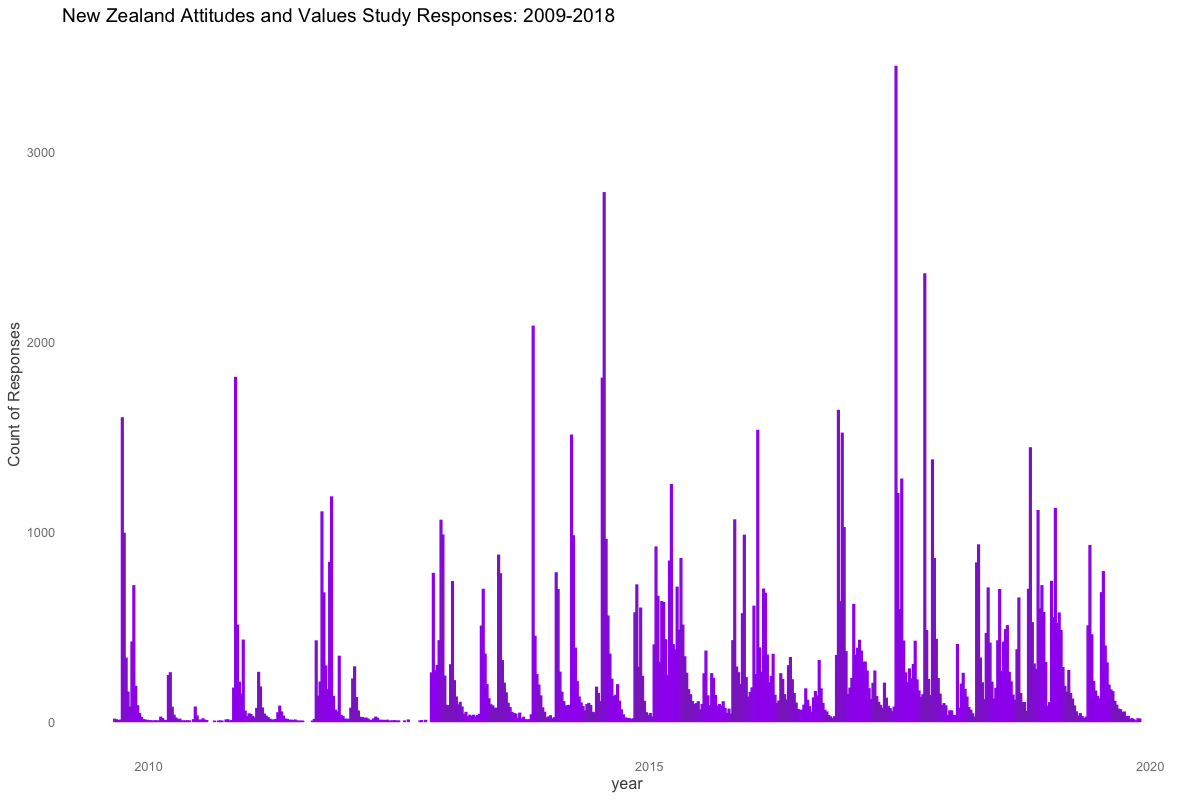
\includegraphics[width=.8\textwidth,height=\textheight,keepaspectratio]{Figures/NZAVSHISTOGRAM.png}
%\caption{}
\end{figure}

\end{frame}


\begin{frame}{Here, we investigate change in (1) Climate Beliefs, (2) Climate Concern, (3) Environmental Efficacy, (4) Sacrificial Behaviour for the Environment in $N = 26,790$ longitudinal participants (responded to two or more waves).}
\begin{block}{Model}
\tiny{
\begin{flalign*}
\sum_{k=1}^{K}\operatorname{Environmental Orientation}_{ij}  &\sim N \left(\mu,\sigma^2 \right) \\ \mu &=\alpha_{j[i]} + \beta_{1}(\operatorname{years}) + \beta_{2}(\operatorname{Relid.S}) + \beta_{3}(\operatorname{Pol.Orient.S})\ + \\
&\quad \beta_{4}(\operatorname{Edu.S}) + \beta_{5}(\operatorname{Age.C.decade}) + \beta_{6}(\operatorname{EthnicCats}_{\operatorname{Māori}}) + \beta_{7}(\operatorname{EthnicCats}_{\operatorname{Pacific}})\ + \\
&\quad \beta_{8}(\operatorname{EthnicCats}_{\operatorname{Asian}}) + \beta_{9}(\operatorname{Male}_{\operatorname{1}}) + \beta_{10}(\operatorname{NZdepS}) + \beta_{11}(\operatorname{Urban}_{\operatorname{1}})\ + \\
&\quad \beta_{12}(\operatorname{years} \times \operatorname{Relid.S}) + \beta_{13}(\operatorname{years} \times \operatorname{Pol.Orient.S}) + \beta_{14}(\operatorname{years} \times \operatorname{Edu.S}) \\ \alpha_{j} &\sim N \left(\mu_{\alpha_{j}},\sigma^2_{\alpha_{j}} \right), \operatorname{ for ~ } i  = 1\dots 26,790 ~\operatorname{Id},  j = 1\dots 10~\operatorname{Waves}
\end{flalign*}
}

\end{block}
\end{frame}

\section{Climate Change Beliefs}
\begin{frame}{1. Climate Change Questions}
    

\begin{alertblock}{~}
"Climate change is real."
\end{alertblock}

\begin{alertblock}{~}
"Climate change is caused by humans."
\end{alertblock}


\end{frame}

\begin{frame}{Trend: in only nine years, there was nearly a 1 point increase in beliefs that climate change is real (!)}
\begin{figure}
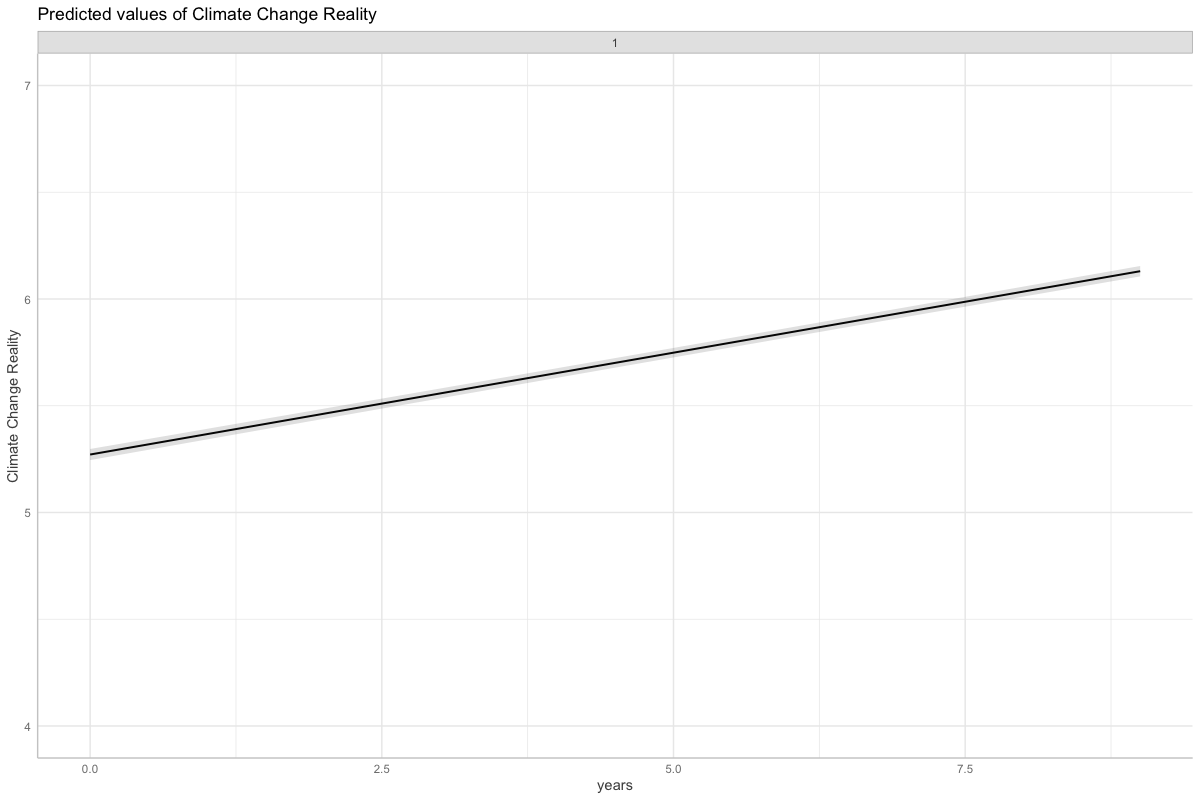
\includegraphics[width=.8\textwidth,height=\textheight,keepaspectratio]{Figures/REAL_TIME.png}
%\caption{}
\end{figure}
\end{frame}


\begin{frame}{Ethnicity: non-Europeans, and especially Pacific/Māori have the strongest climate beliefs (panels show years 2009,2013,2018).}
\begin{figure}
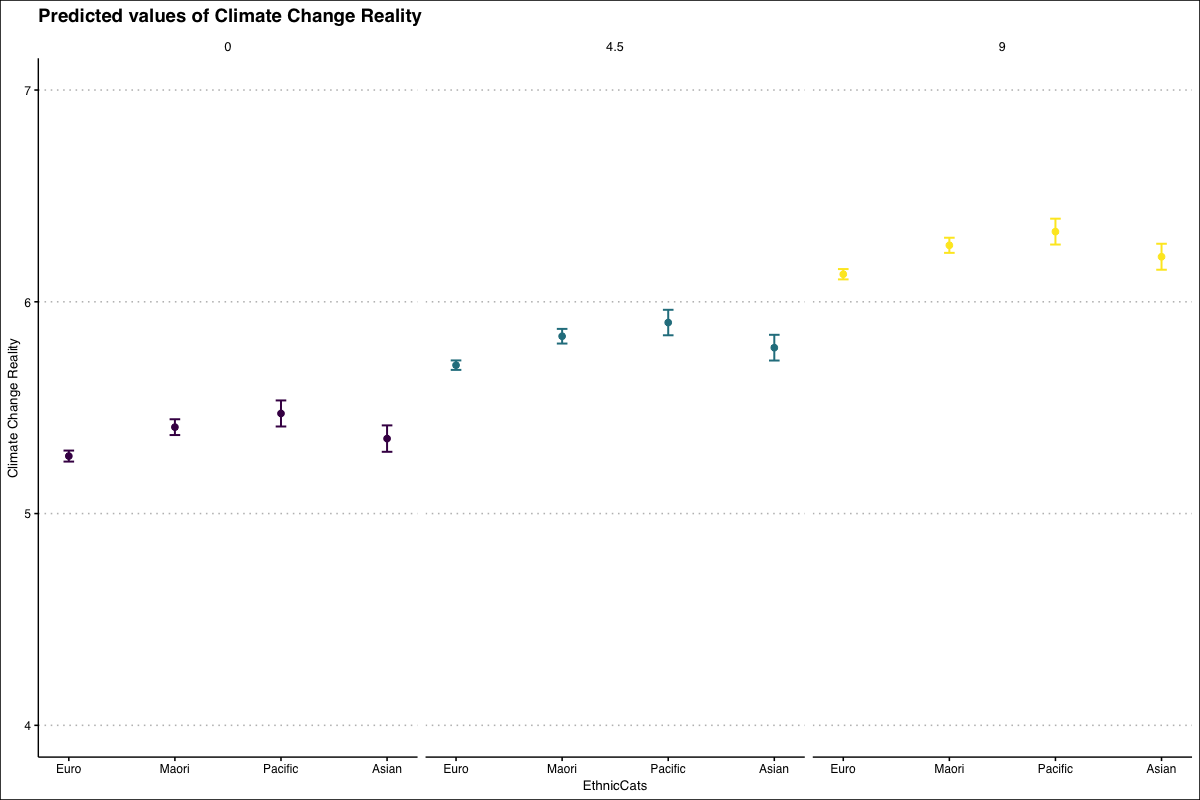
\includegraphics[width=.8\textwidth,height=\textheight,keepaspectratio]{Figures/REAL_EthnicCats_T.png}
%\caption{}
\end{figure}
\end{frame}


\begin{frame}{Education: the relationship between education and climate change beliefs has strengthened.}
\begin{figure}
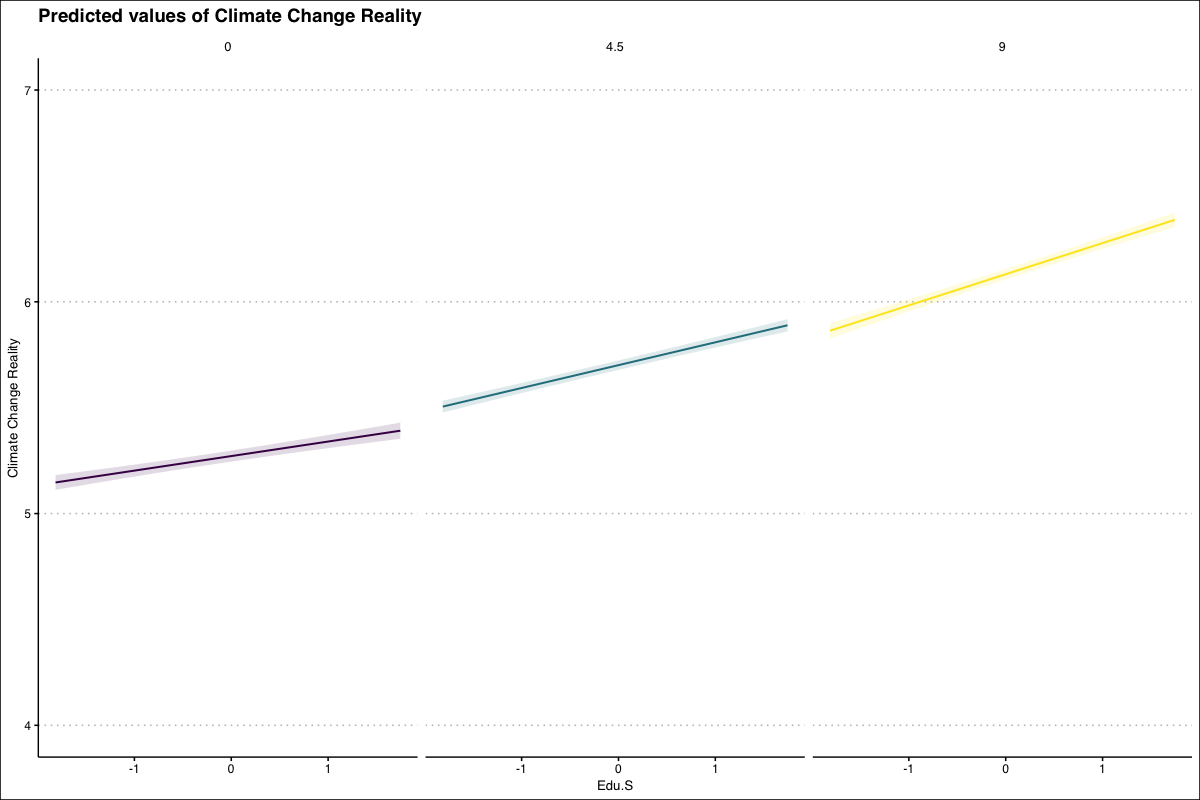
\includegraphics[width=.8\textwidth,height=\textheight,keepaspectratio]{Figures/REAL_Edu.S.png}
%\caption{
\end{figure}
\end{frame}

\begin{frame}{Political conservatism predicts weaker beliefs in climate change, however conservatives are more convinced of climate change than were liberals were a decade ago.}
\begin{figure}
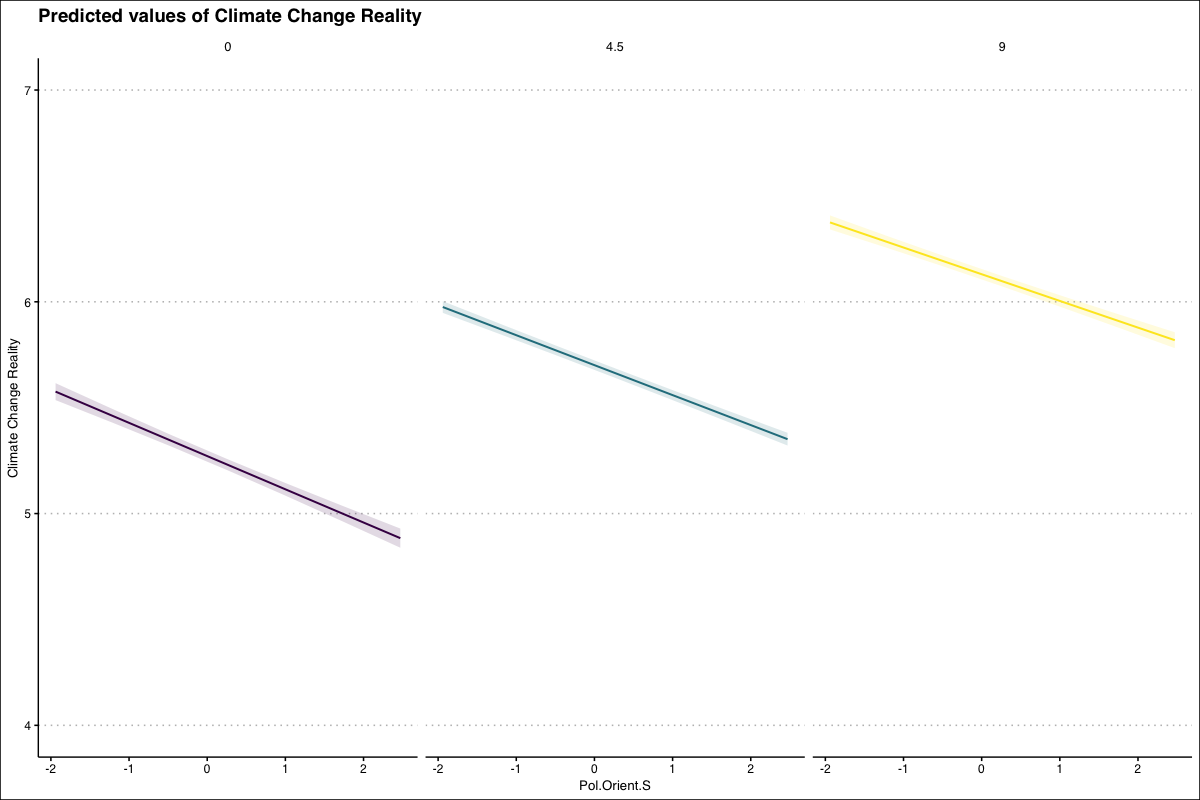
\includegraphics[width=.8\textwidth,height=\textheight,keepaspectratio]{Figures/REAL_Pol.Orient.S.png}
%\caption{}
\end{figure}
\end{frame}

\begin{frame}{Religious people have also increasingly accepted climate change, but religious identification is increasingly attenuating such beliefs.}
\begin{figure}
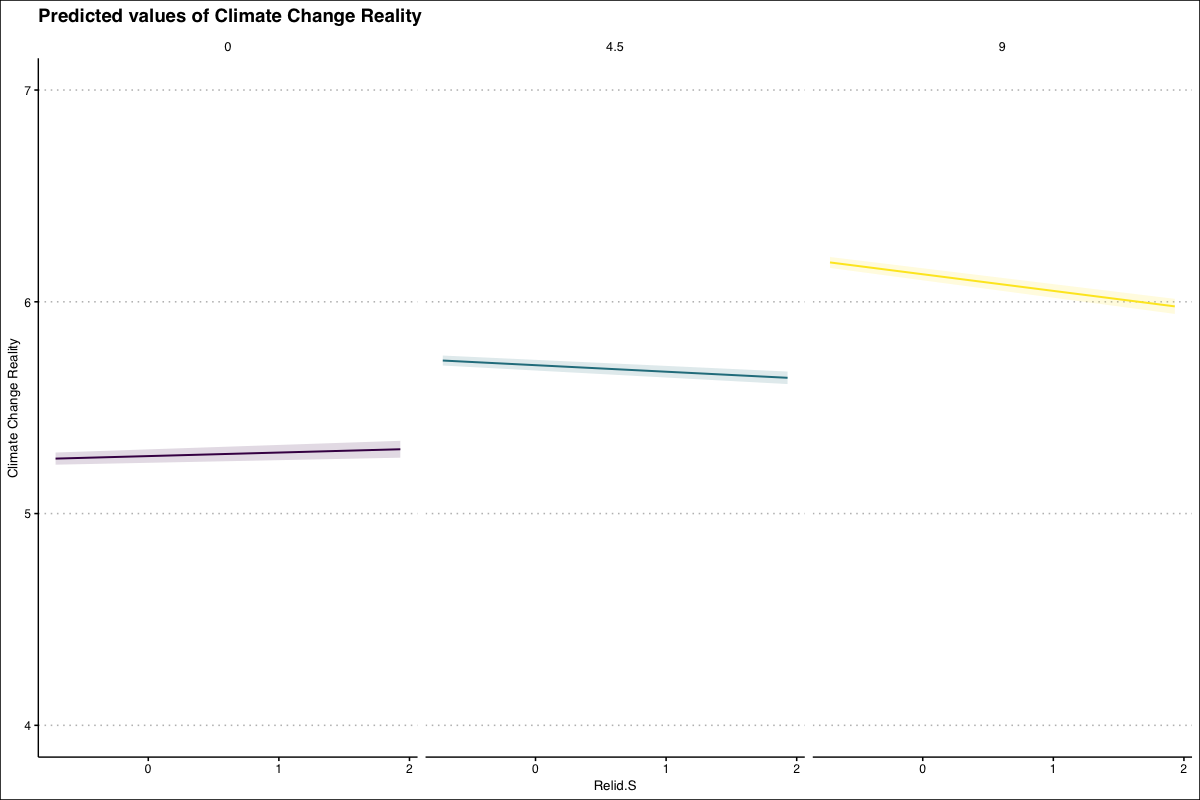
\includegraphics[width=.8\textwidth,height=\textheight,keepaspectratio]{Figures/REAL_RELIDS_T.png}
%\caption{}
\end{figure}
\end{frame}

% \begin{frame}{Religion  Climate Change is Human Caused}
% \begin{figure}
% 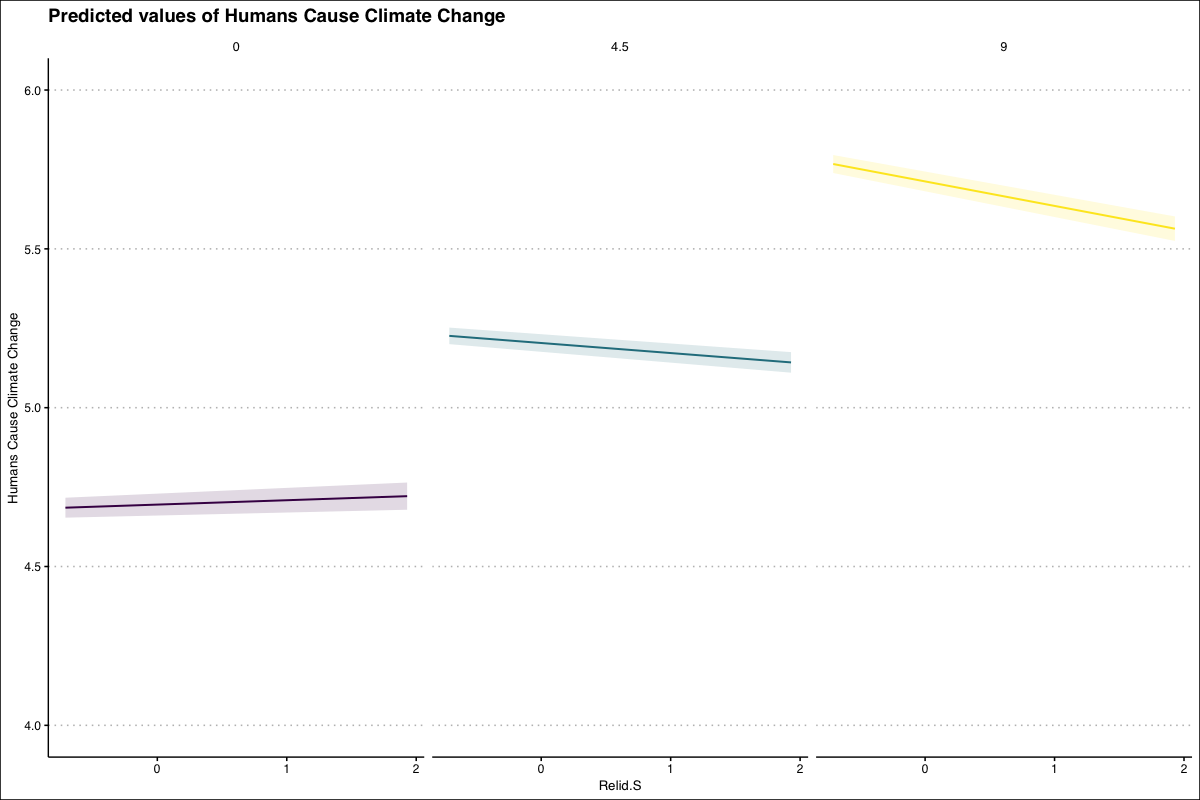
\includegraphics[width=.99\textwidth,height=\textheight,keepaspectratio]{Figures/HUMANCAUSED_RELIDS_T.png}
% %\caption{}
% \end{figure}
% \end{frame}

\section{Concern about Climate}
\begin{frame}{2. Climate Concern Question (2013-2018}
    

\begin{alertblock}{~}
"I am deeply concerned about climate change."
\end{alertblock}

\end{frame}


\begin{frame}{Trend: during the past five years, there has been a strong increase in concern about climate (about 1/2 point)}
\begin{figure}
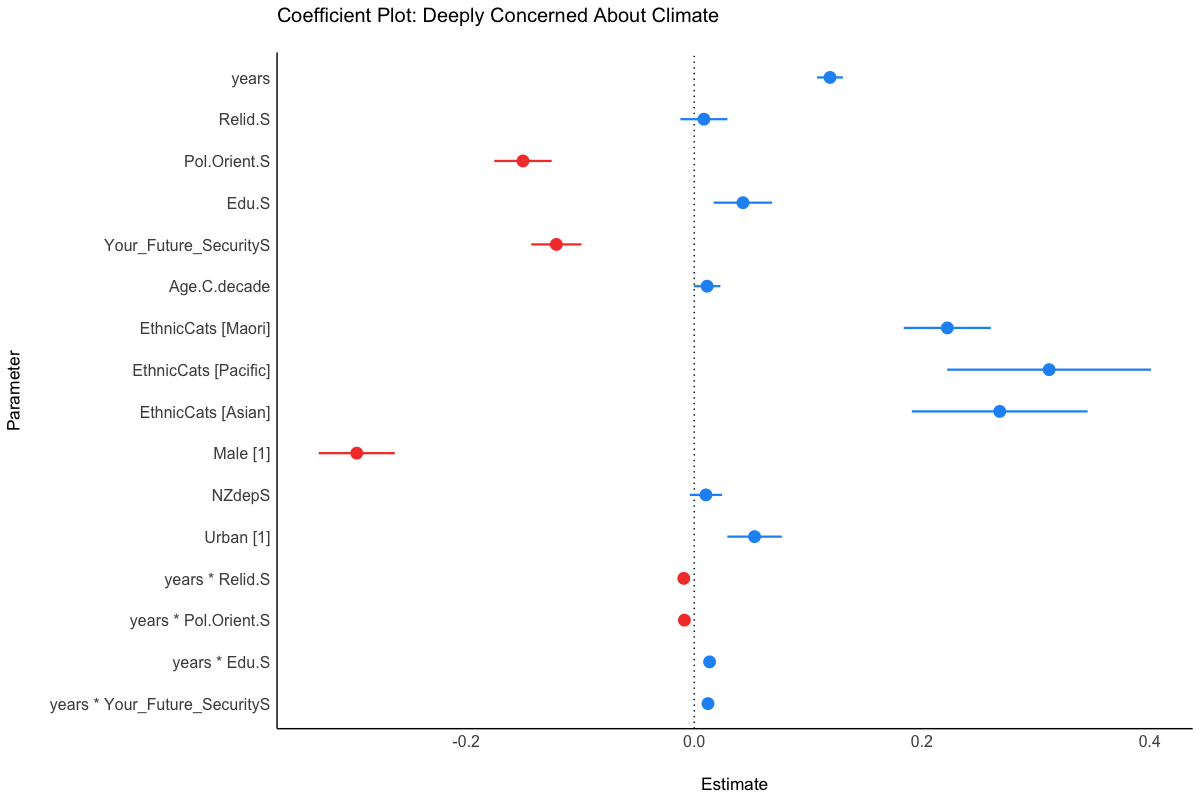
\includegraphics[width=.8\textwidth,height=\textheight,keepaspectratio]{Figures/CONCERN_TIME.png}
%\caption{}
\end{figure}
\end{frame}


\begin{frame}{Ethnicity: Europeans are substantially less concerned about climate than are other ethnic groups}
\begin{figure}
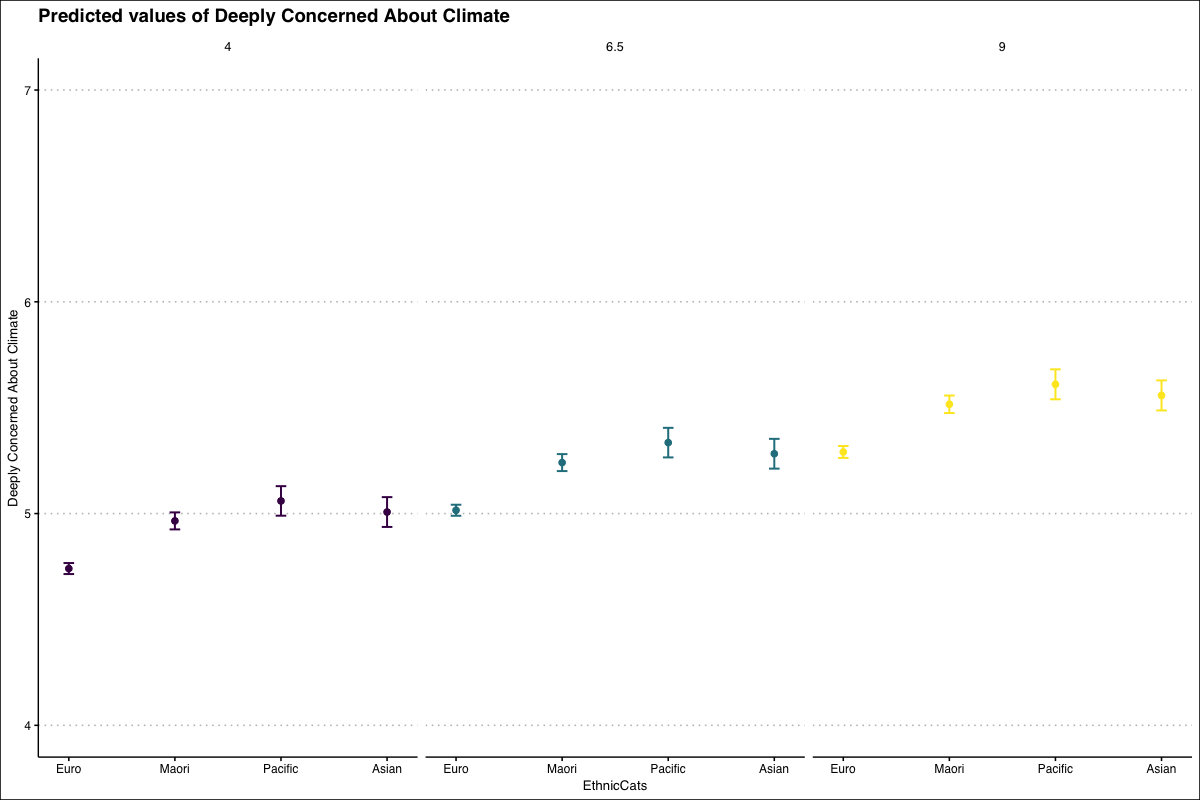
\includegraphics[width=.8\textwidth,height=\textheight,keepaspectratio]{Figures/CONCERN_EthnicCats_T.png}
%\caption{}
\end{figure}
\end{frame}


\begin{frame}{Education: the relationship between education and climate concern has increased.}
\begin{figure}
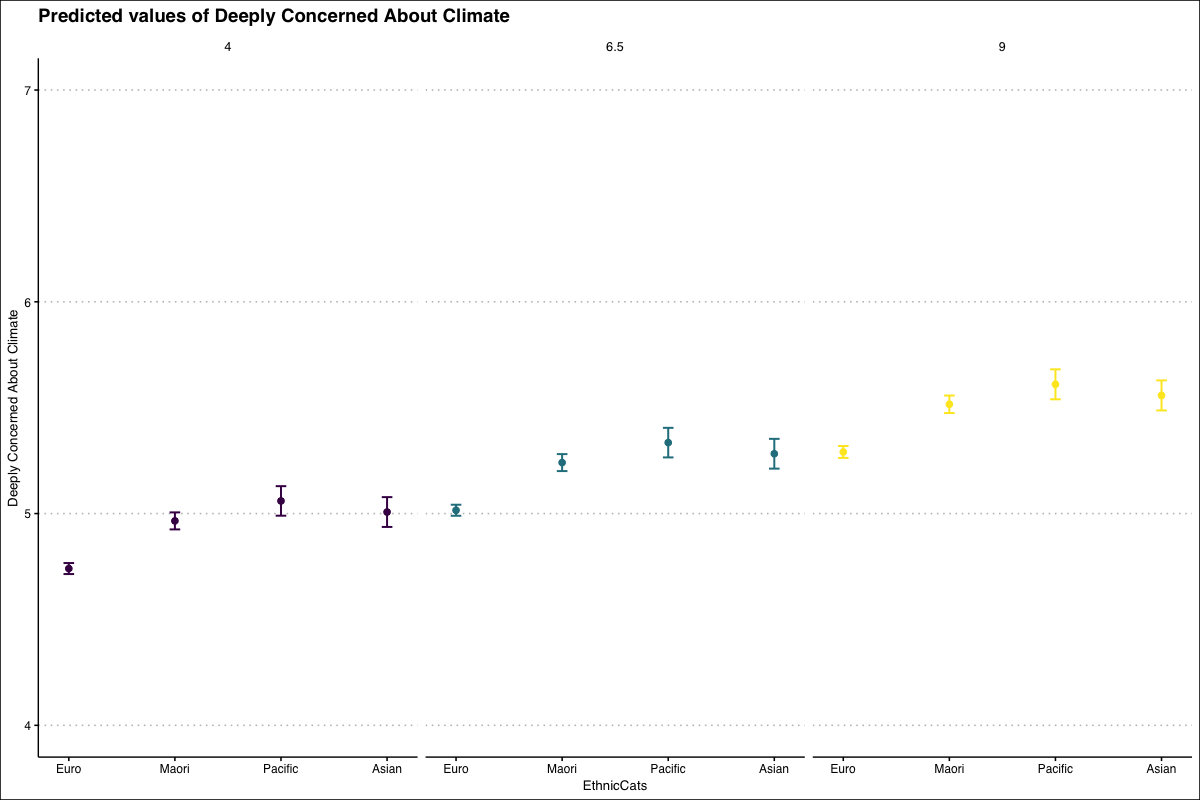
\includegraphics[width=.8\textwidth,height=\textheight,keepaspectratio]{Figures/CONCERN_Edu.S.png}
%\caption{}
\end{figure}
\end{frame}


\begin{frame}{Political Conservativism strongly attenuates climate concern (even as conservatives accept climate change is real.)}
\begin{figure}
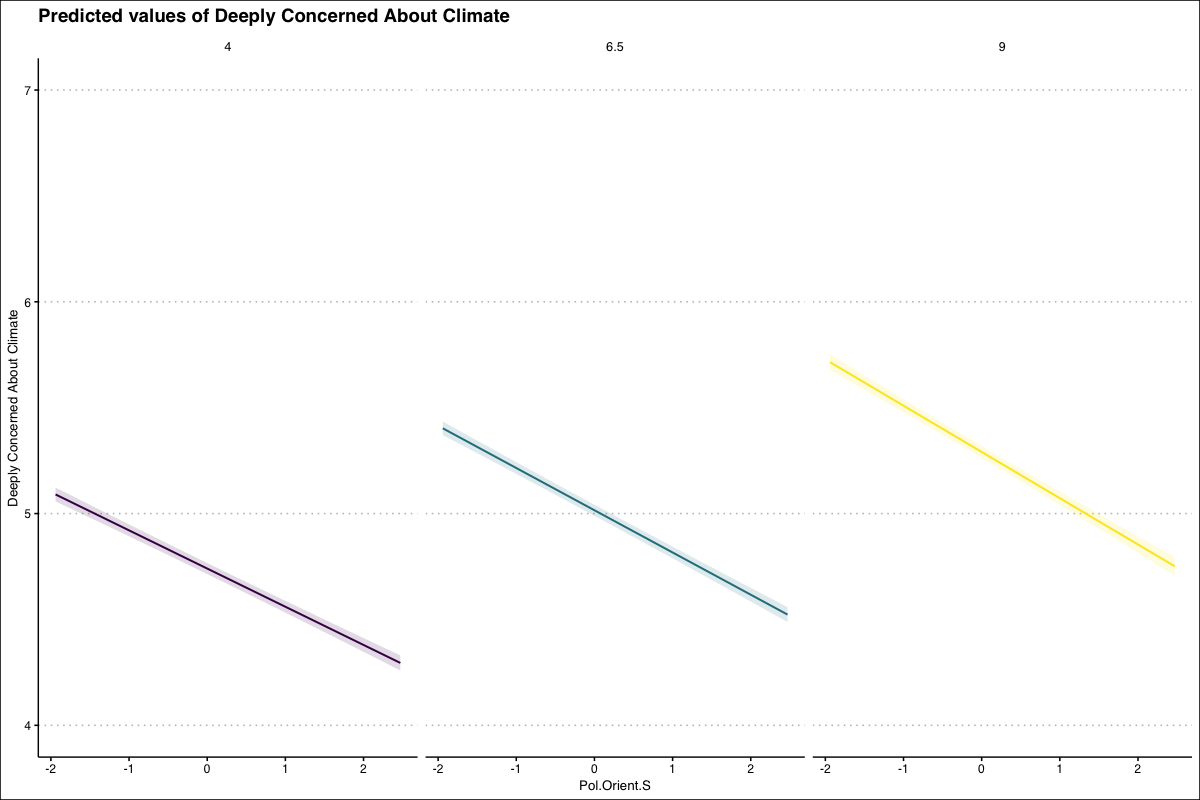
\includegraphics[width=.8\textwidth,height=\textheight,keepaspectratio]{Figures/CONCERN_Pol.Orient.S.png}
%\caption{}
\end{figure}
\end{frame}


\begin{frame}{Religious people have grown in climate concern, but religious identification is increasingly suppressing environmental concern}
\begin{figure}
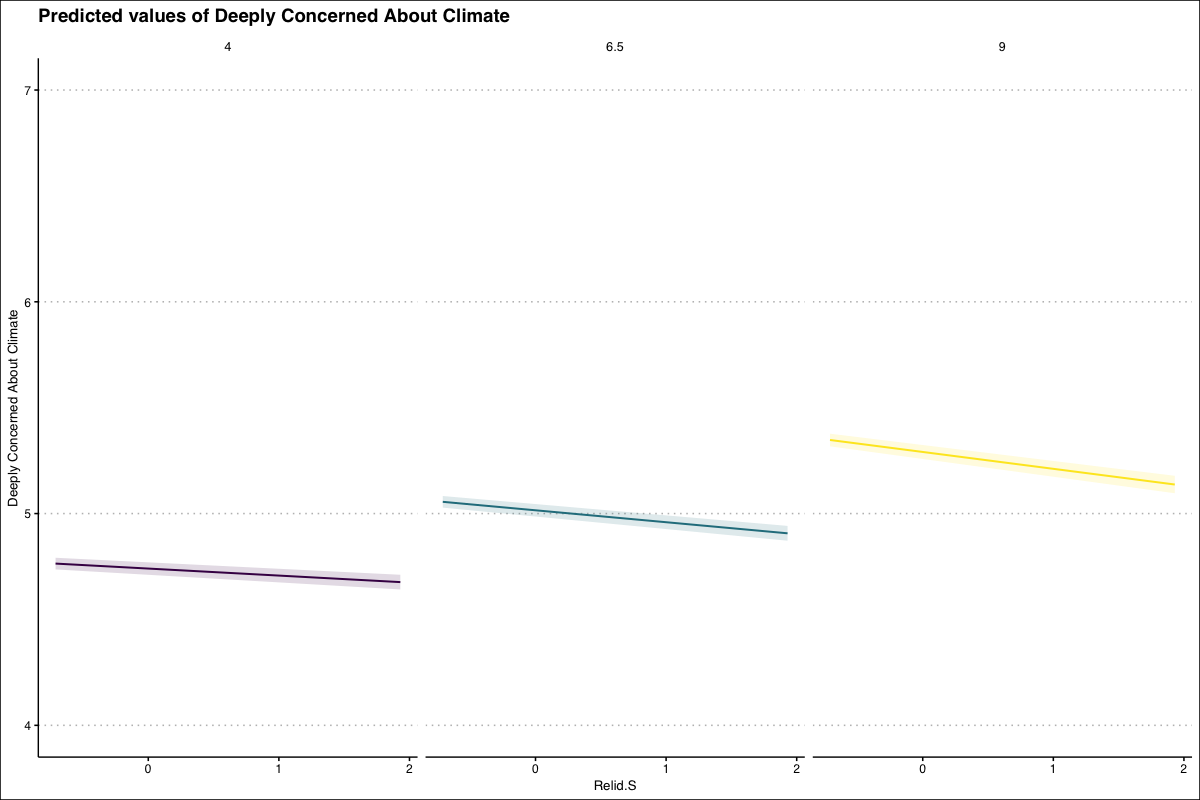
\includegraphics[width=.8\textwidth,height=\textheight,keepaspectratio]{Figures/CONCERN_RELIDS_T.png}
%\caption{}
\end{figure}
\end{frame}


\section{Beliefs My Behavior Can Help The Environment}
\begin{frame}{3. Environmental Efficacy Questions}
    

\begin{alertblock}{~}
"By taking personal action I believe I can make a positive difference to environmental problems."
\end{alertblock}

\begin{alertblock}{~}
"I feel I can make a difference to the state of the environment."
\end{alertblock}

\end{frame}

\begin{frame}{Trend: beliefs in environmental efficacy are slowly increasing}
\begin{figure}
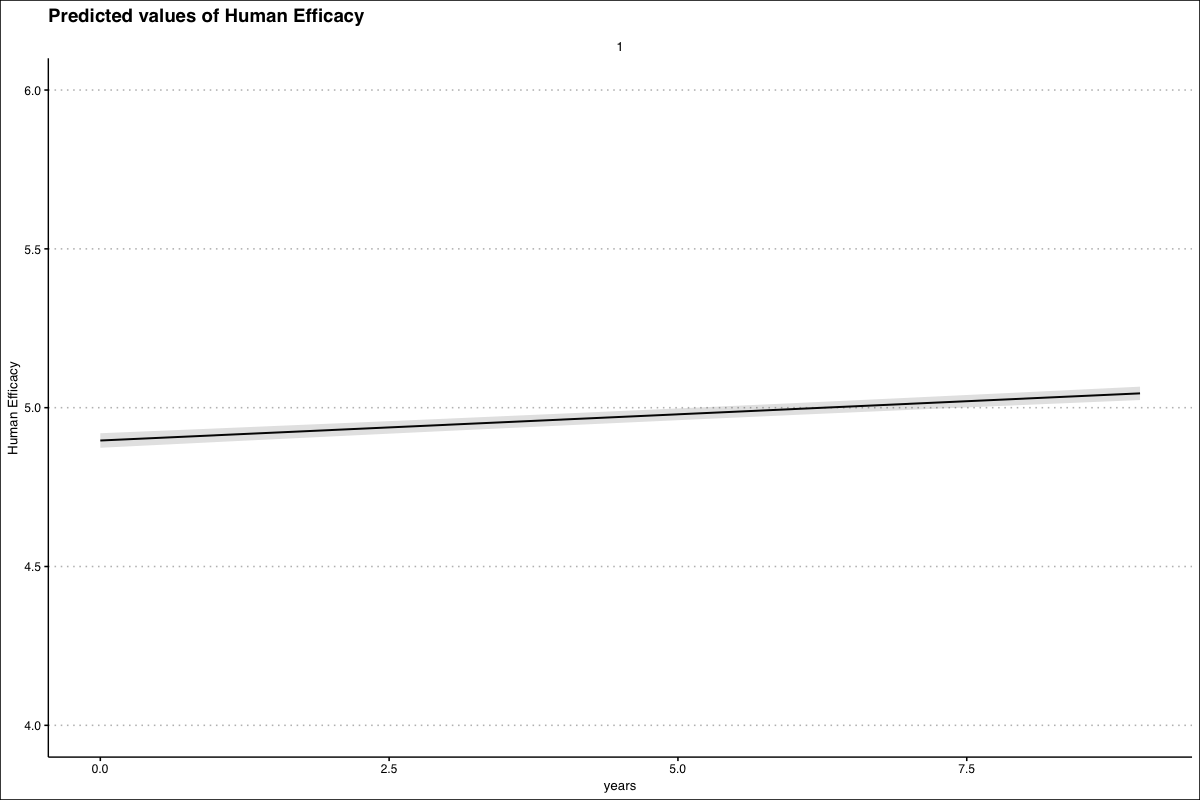
\includegraphics[width=.8\textwidth,height=\textheight,keepaspectratio]{Figures/EFFICACY_TIME.png}
%\caption{}
\end{figure}
\end{frame}

\begin{frame}{Ethnicity: Pakeha are only now catching up with Māori a decade ago in environmental efficacy beliefs}
\begin{figure}
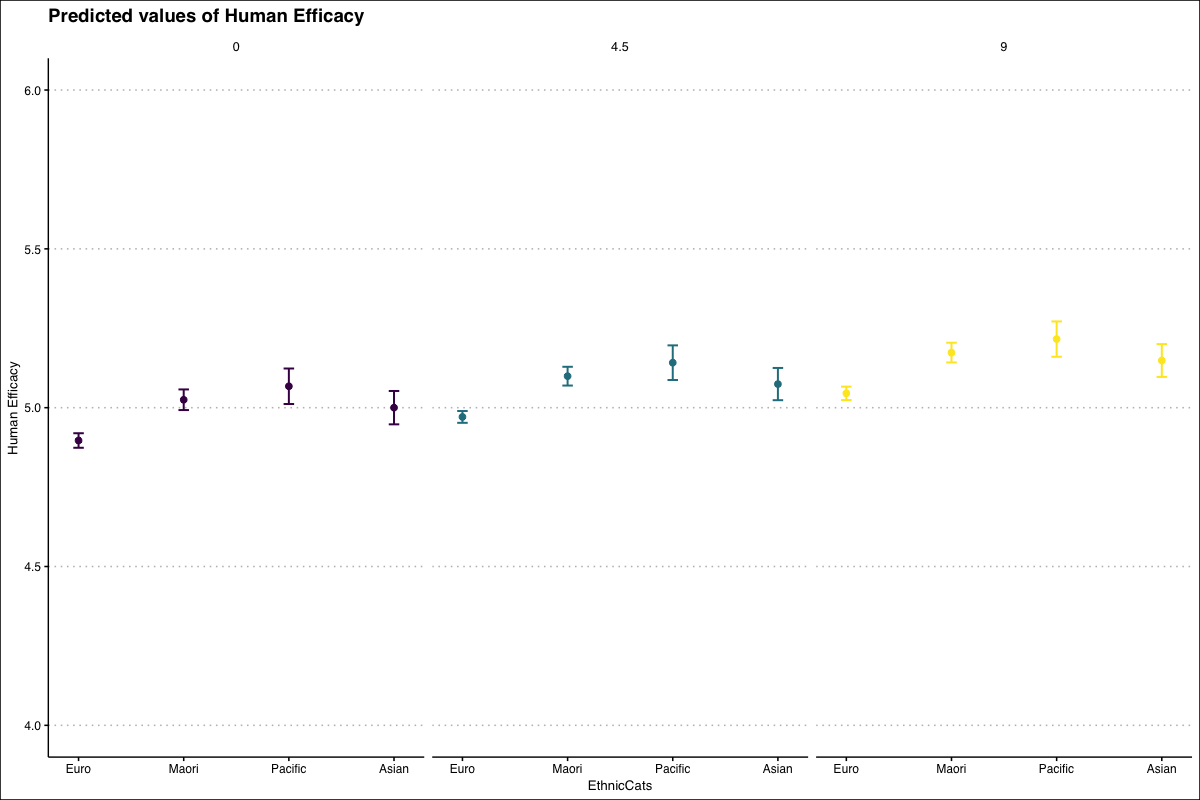
\includegraphics[width=.8\textwidth,height=\textheight,keepaspectratio]{Figures/EFFICACY_EthnicCats_T.png}
%\caption{}
\end{figure}
\end{frame}


\begin{frame}{Education: the relationship of education to environmental efficacy beliefs is becoming increasingly important.}
\begin{figure}
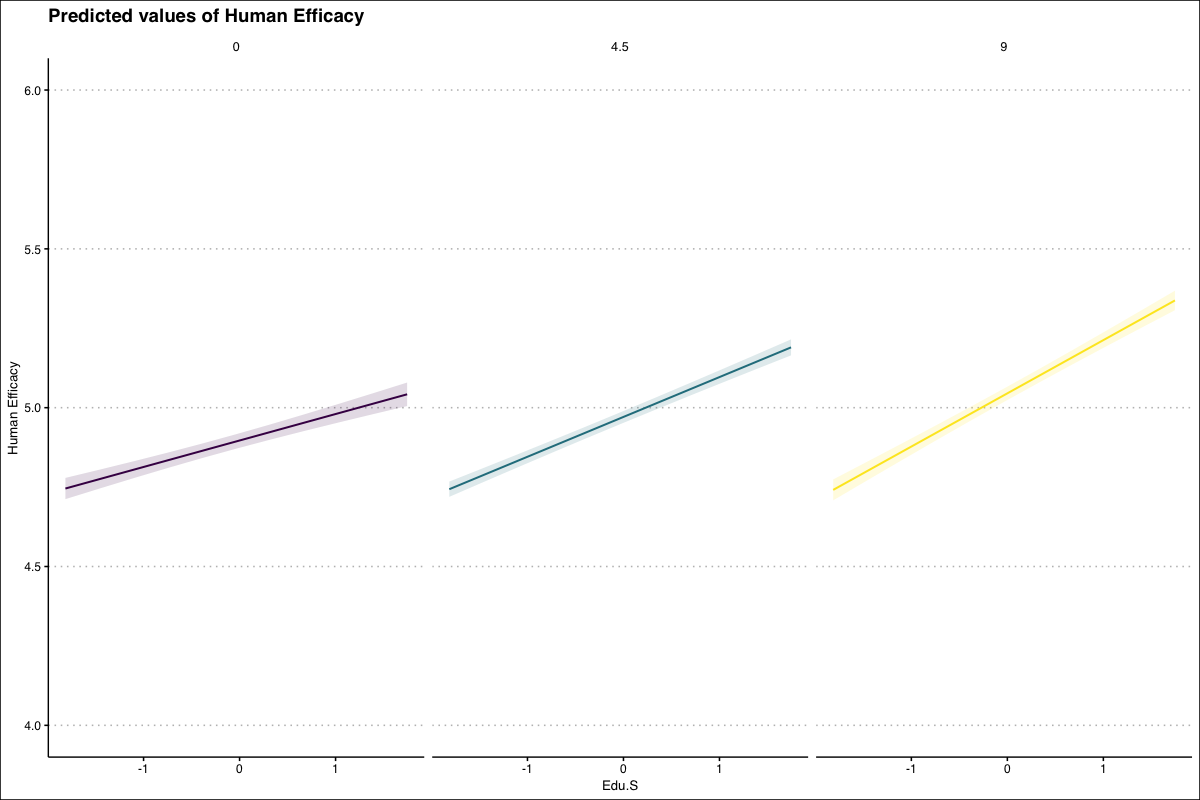
\includegraphics[width=.8\textwidth,height=\textheight,keepaspectratio]{Figures/EFFICACY_Edu.S.png}
%\caption{}
\end{figure}
\end{frame}


\begin{frame}{Political Conservativism  predicts {\bf weaker} environmental efficacy beliefs.}
\begin{figure}
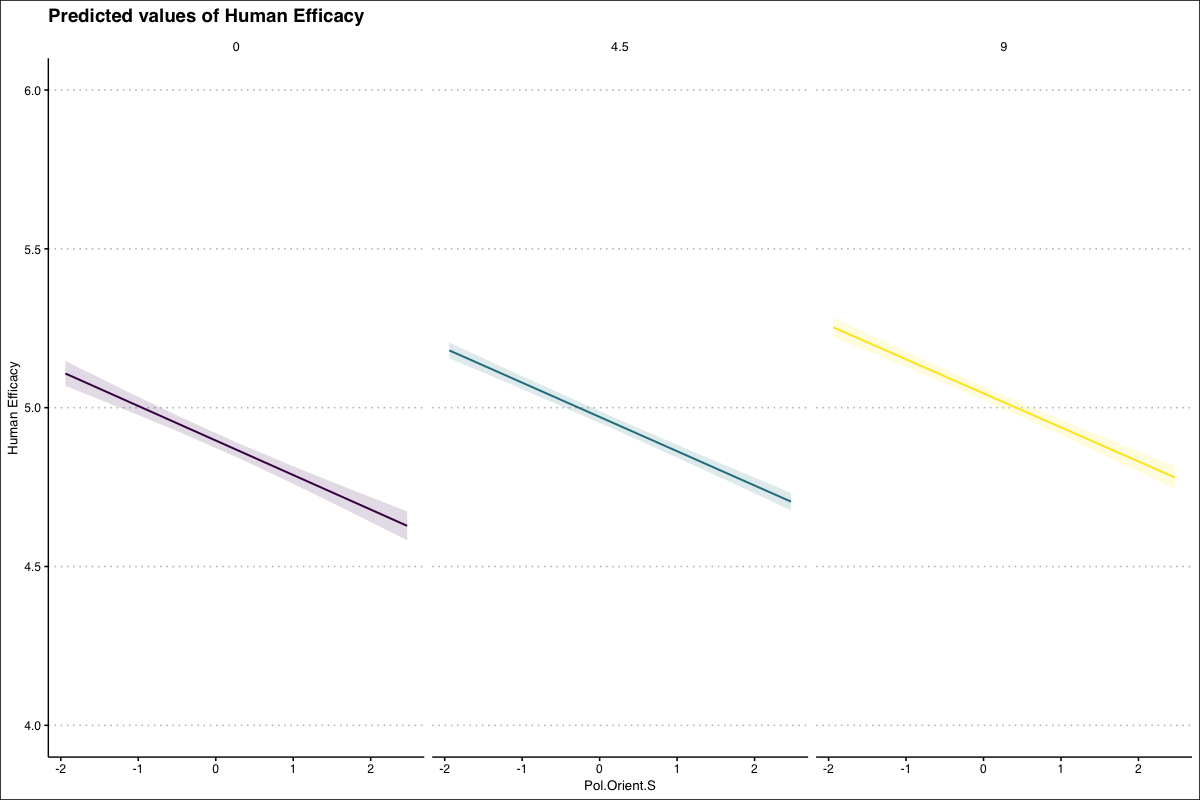
\includegraphics[width=.8\textwidth,height=\textheight,keepaspectratio]{Figures/EFFICACY_Pol.Orient.S.png}
%\caption{}
\end{figure}
\end{frame}


\begin{frame}{Religion has long been associated with {\bf stronger} environmental efficacy beliefs, however the relationship is weakening}
\begin{figure}
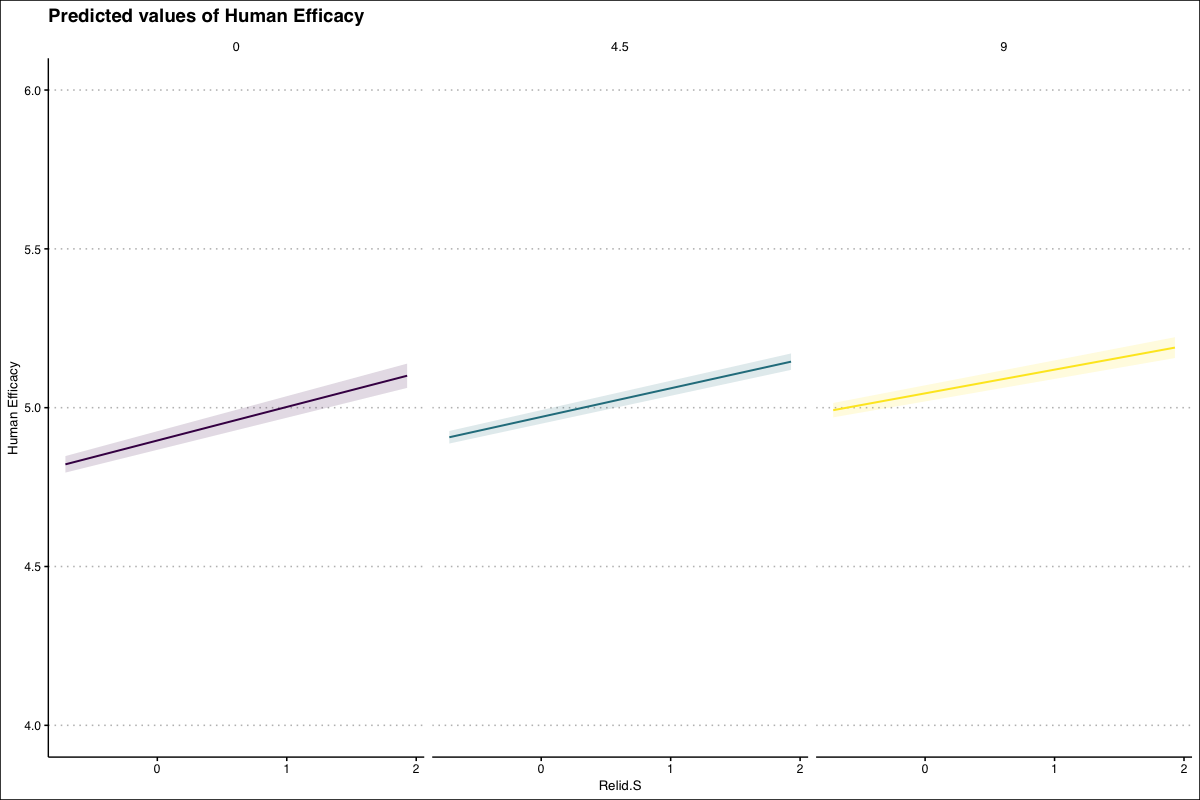
\includegraphics[width=.8\textwidth,height=\textheight,keepaspectratio]{Figures/EFFICACY_RELIDS_T.png}
%\caption{}
\end{figure}
\end{frame}


\section{Sacrificial Behaviour for the Environment}
\begin{frame}{4. Climate Sacrifice Questions}
    

\begin{alertblock}{~}
"Have you made sacrifices to your standard of living (e.g., accepted higher prices, driven less, conserved energy) in order to protect the environment?"
\end{alertblock}

% \begin{alertblock}{~}
% "Have you made changes to your daily routine in order to protect the environment?"
% \end{alertblock}

\end{frame}



\begin{frame}{Trend: there has not been much increase in environmental sacrificial behaviors.}
\begin{figure}
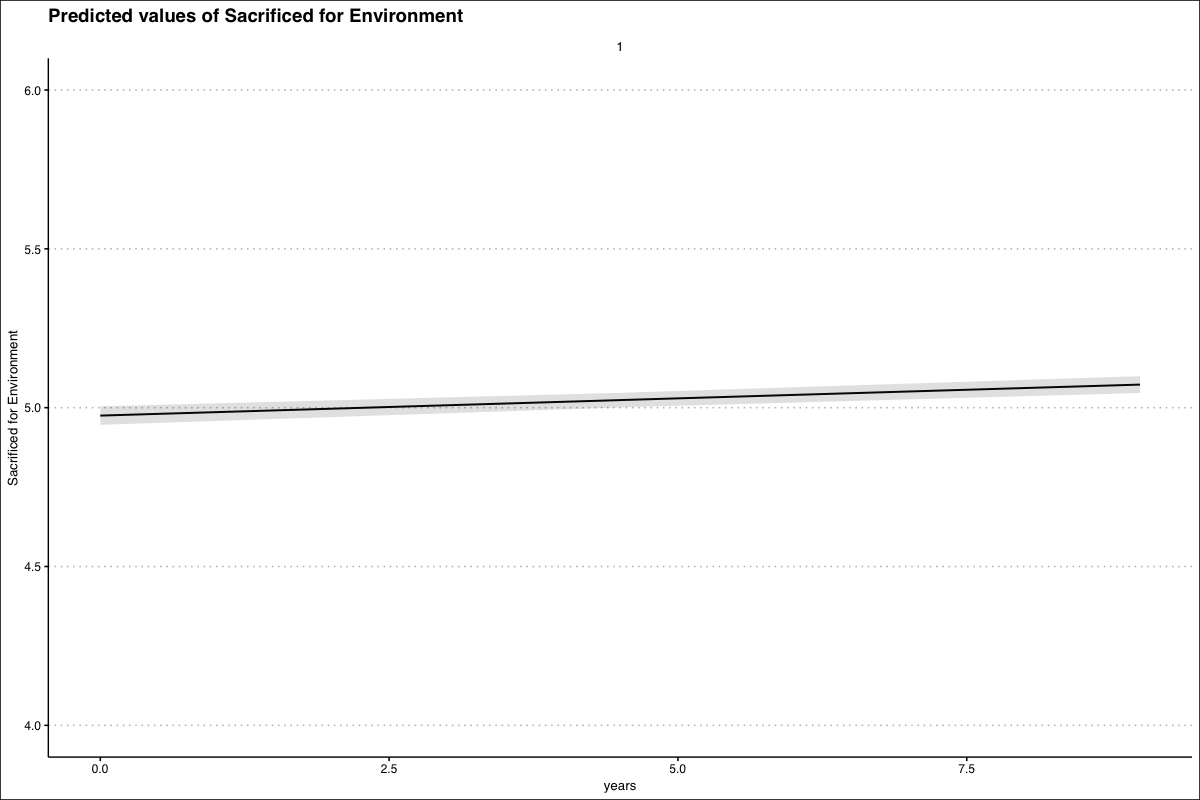
\includegraphics[width=.8\textwidth,height=\textheight,keepaspectratio]{Figures/SACRIFICEMADE_TIME.png}
%\caption{}
\end{figure}
\end{frame}

\begin{frame}{Ethnicity: Māori sacrifice more for the environment, and Pakeha have yet to catch up}
\begin{figure}
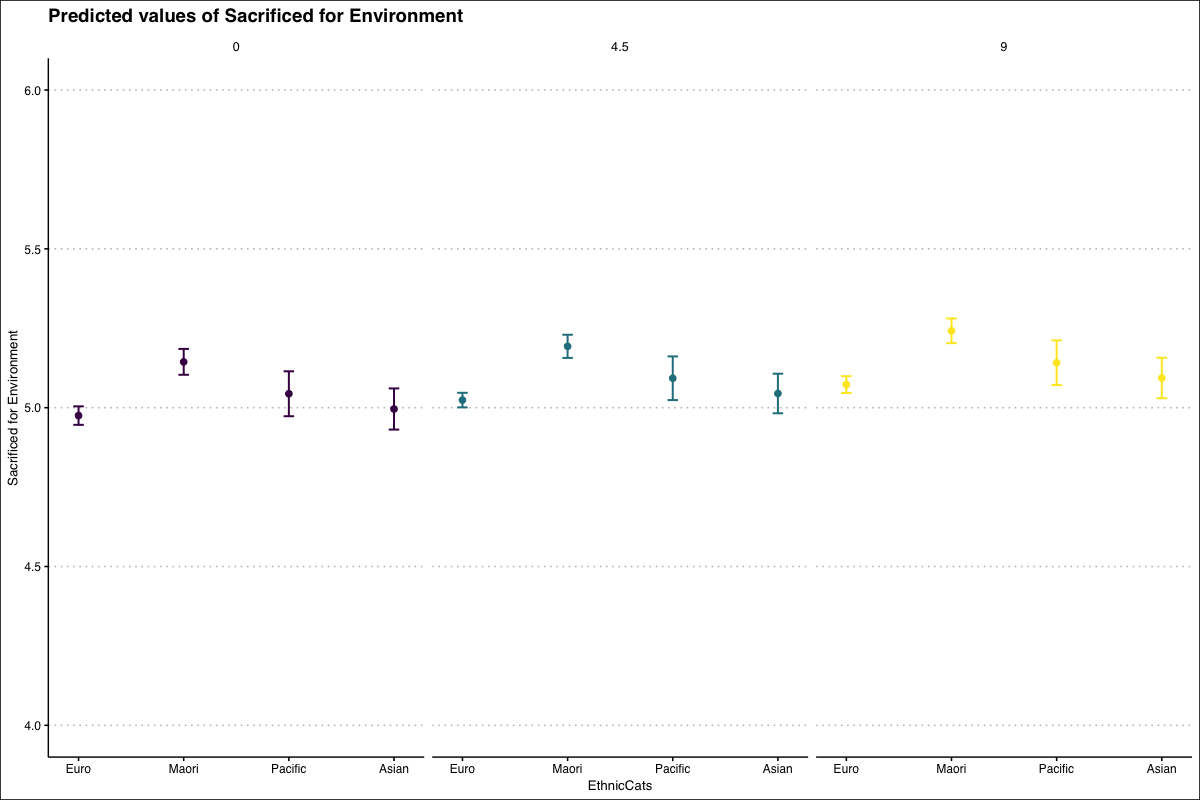
\includegraphics[width=.8\textwidth,height=\textheight,keepaspectratio]{Figures/SACRIFICEMADE_EthnicCats_T.png}
%\caption{}
\end{figure}
\end{frame}

\begin{frame}{Education: the relationship between education and environmental sacrifice is becoming more important; those low in education are sacrificing {\bf less} now than a decade ago.}
\begin{figure}
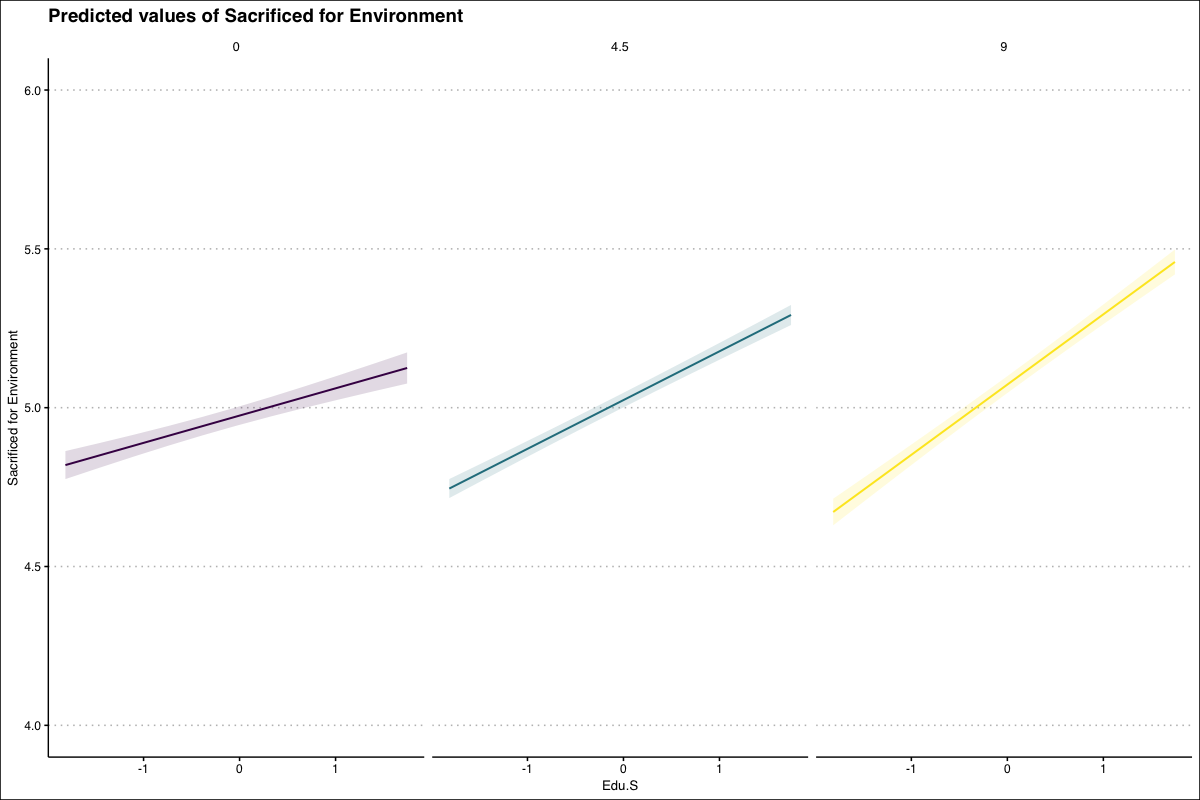
\includegraphics[width=.8\textwidth,height=\textheight,keepaspectratio]{Figures/SACRIFICEMADE_Edu.S.png}
%\caption{}
\end{figure}
\end{frame}


\begin{frame}{Political Conservativism predicts {\bf lower} environmental sacrifice, with all of the growth occurring among political liberals}
\begin{figure}
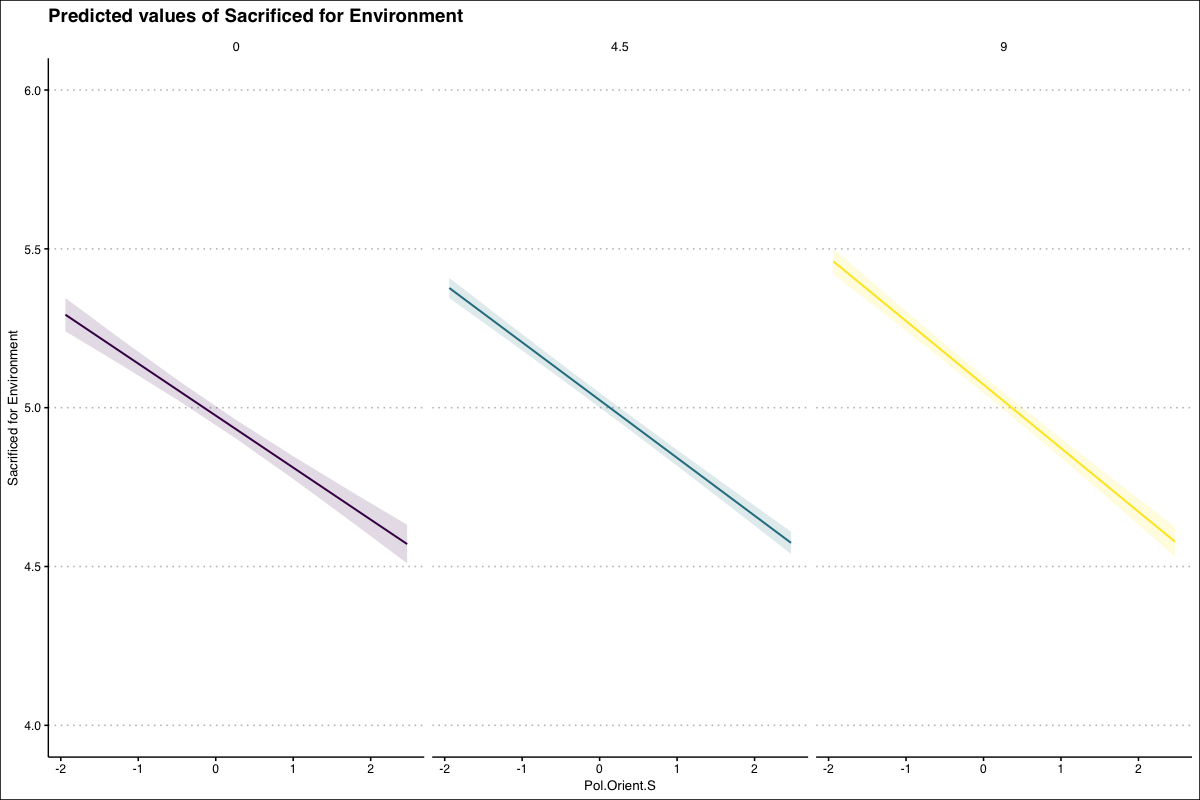
\includegraphics[width=.8\textwidth,height=\textheight,keepaspectratio]{Figures/SACRIFICEMADE_Pol.Orient.S.png}
%\caption{}
\end{figure}
\end{frame}


\begin{frame}{Religion has long been associated with {\bf stronger} environmental efficacy beliefs, however the relationship is weakening.}
\begin{figure}
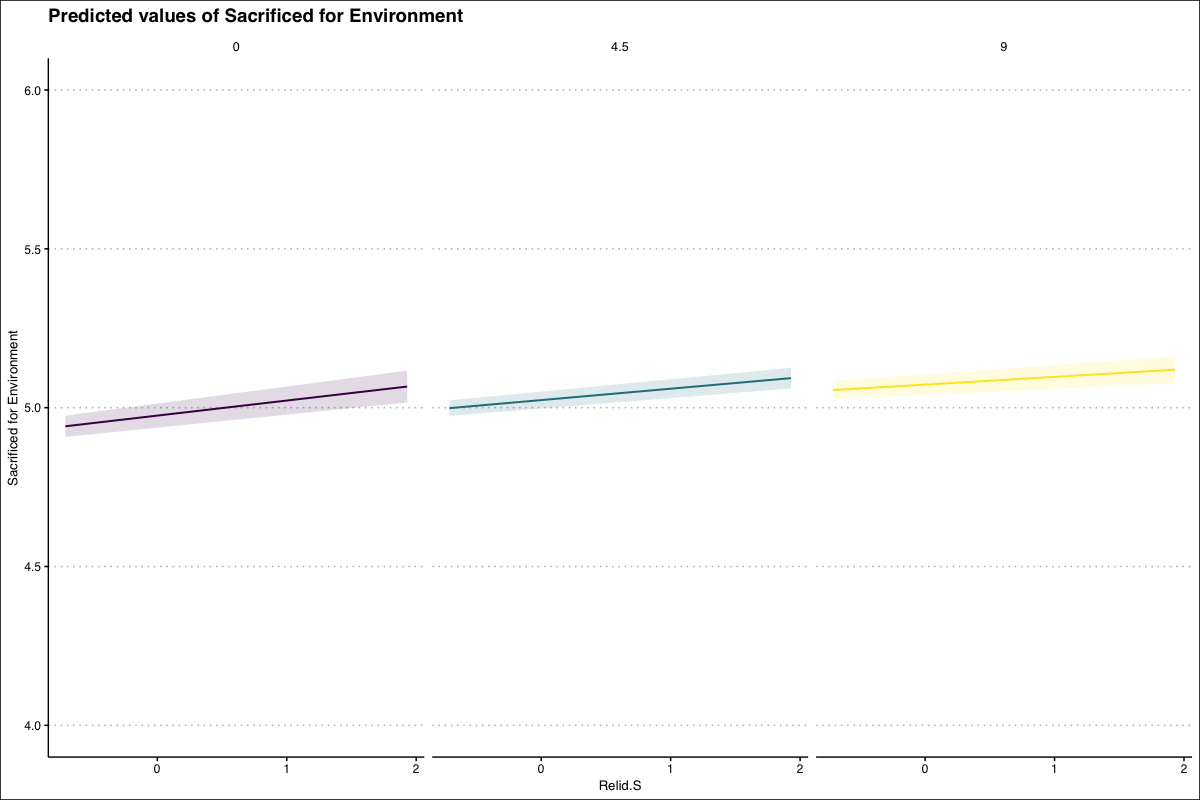
\includegraphics[width=.8\textwidth,height=\textheight,keepaspectratio]{Figures/SACRIFICEMADE_RELIDS_T.png}
%\caption{}
\end{figure}
\end{frame}

\section{What Motivates Sacrifice for the Environment?}
\begin{frame}{How do ideologies and emotions combine to motivate environmental sacrifice?}
    

\begin{alertblock}{Future (in)Security}
"Satisfied with my future security."
\end{alertblock}


\begin{alertblock}{(dis)Satisfaction with New Zealand's environment}
Satisfaction with quality of New Zealand's natural environment.
\end{alertblock}

% \begin{alertblock}{~}
% "Have you made changes to your daily routine in order to protect the environment?"
% \end{alertblock}

\end{frame}


\begin{frame}{Political Conservativism: future (in)security and does not predict greater environmental sacrifice.}
\begin{figure}
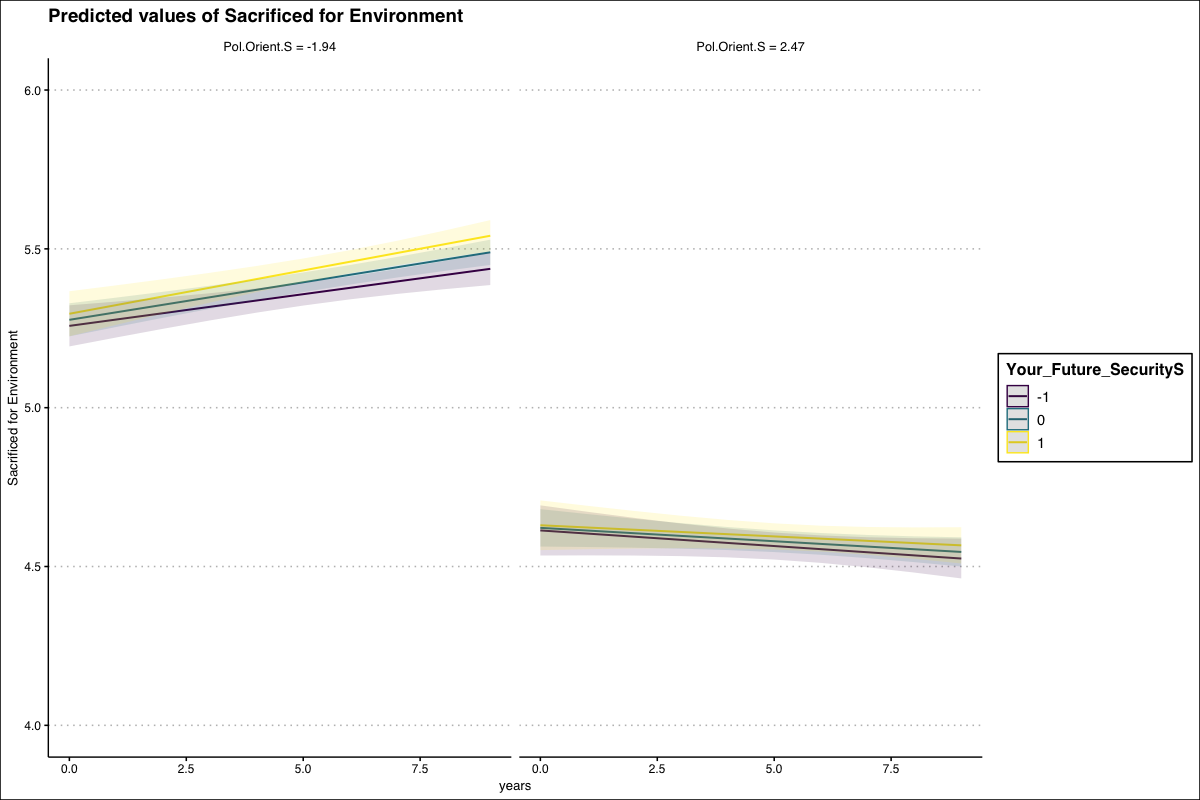
\includegraphics[width=.8\textwidth,height=\textheight,keepaspectratio]{Figures/X_SACRIFICEMADE_Your_Future_SecurityS_Pol.Orient.S.png}
%\caption{}
\end{figure}
\end{frame}

\begin{frame}{Religious Identification: future (in)security  does not predict greater environmental sacrifice}
\begin{figure}
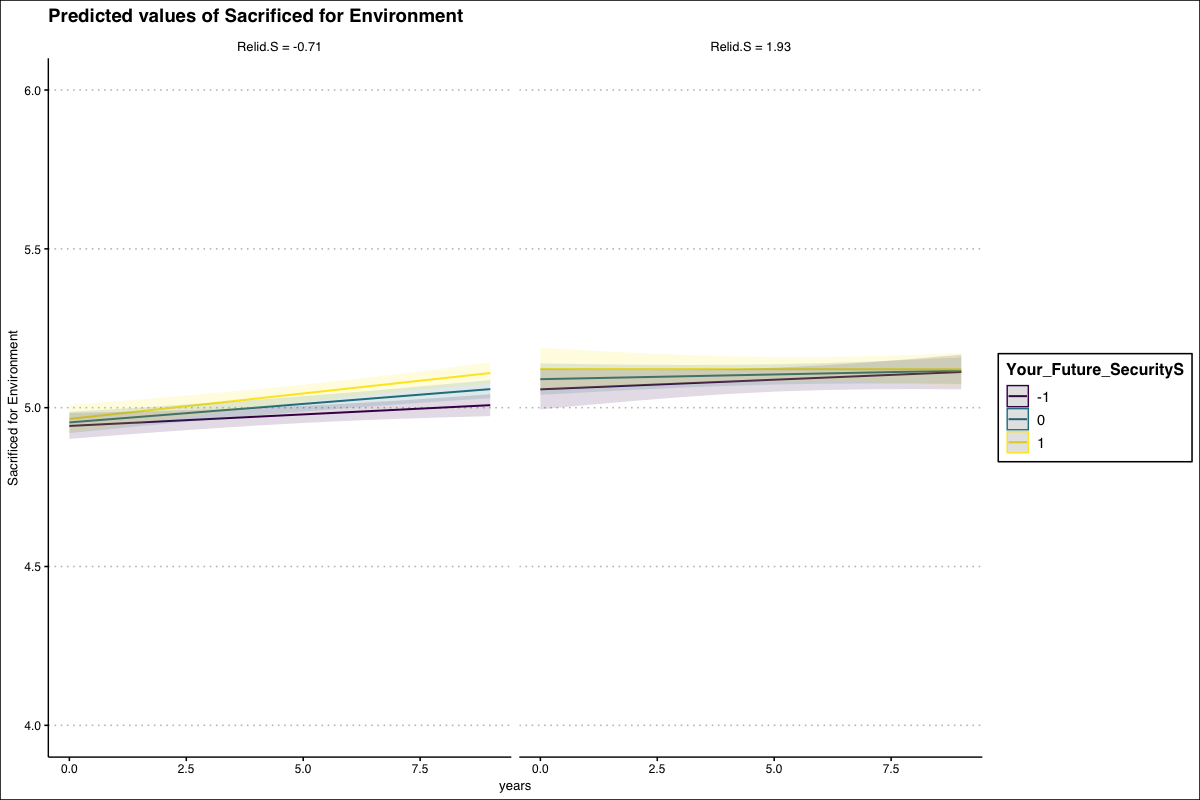
\includegraphics[width=.8\textwidth,height=\textheight,keepaspectratio]{Figures/X_SACRIFICEMADE_Your_Future_SecurityS_Relid.S.png}
%\caption{}
\end{figure}
\end{frame}

\begin{frame}{(dis)Satisfaction with the environment predicts greater environmental sacrifice at low and high levels of Political Conservativism.}
\begin{figure}
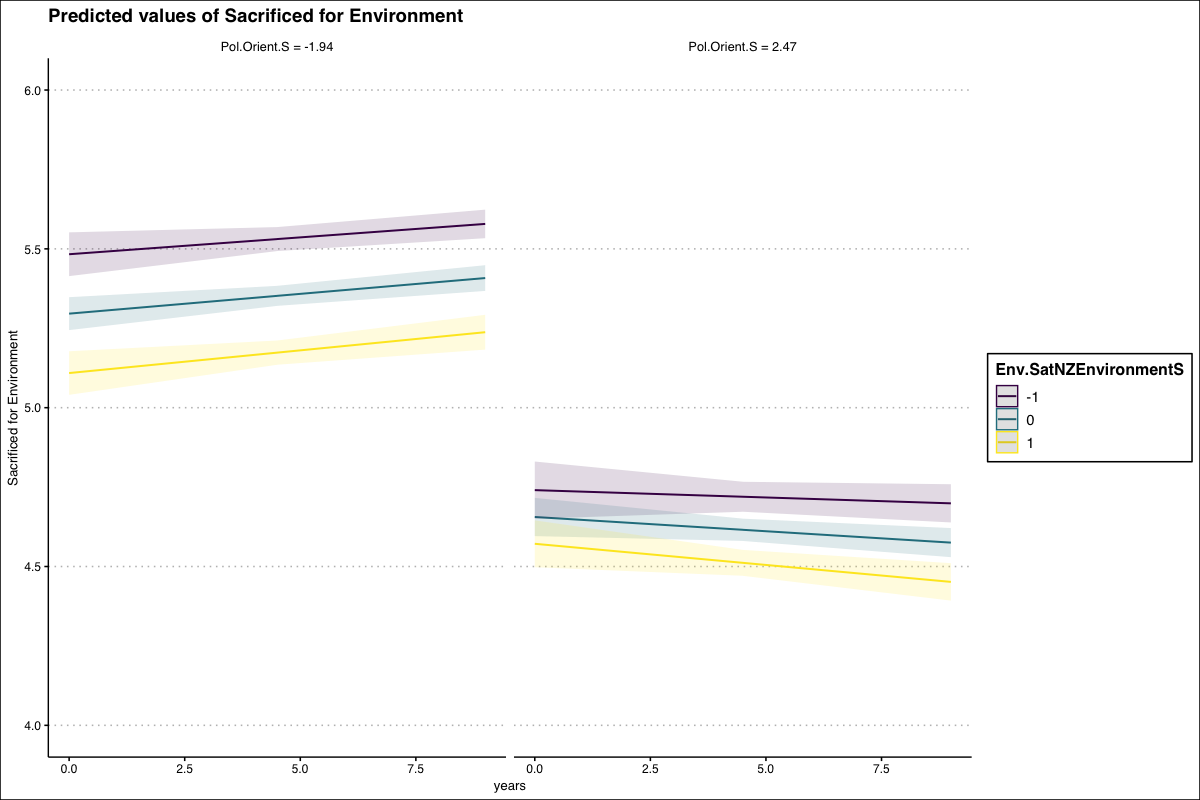
\includegraphics[width=.8\textwidth,height=\textheight,keepaspectratio]{Figures/X_SACRIFICEMADE_Env.SatNZEnvironmentS_Pol.Orient.S.png}
%\caption{}
\end{figure}
\end{frame}

\begin{frame}{(dis)Satisfaction with the environment predicts greater environmental sacrifice at low and high level of Religious Identification.}
\begin{figure}
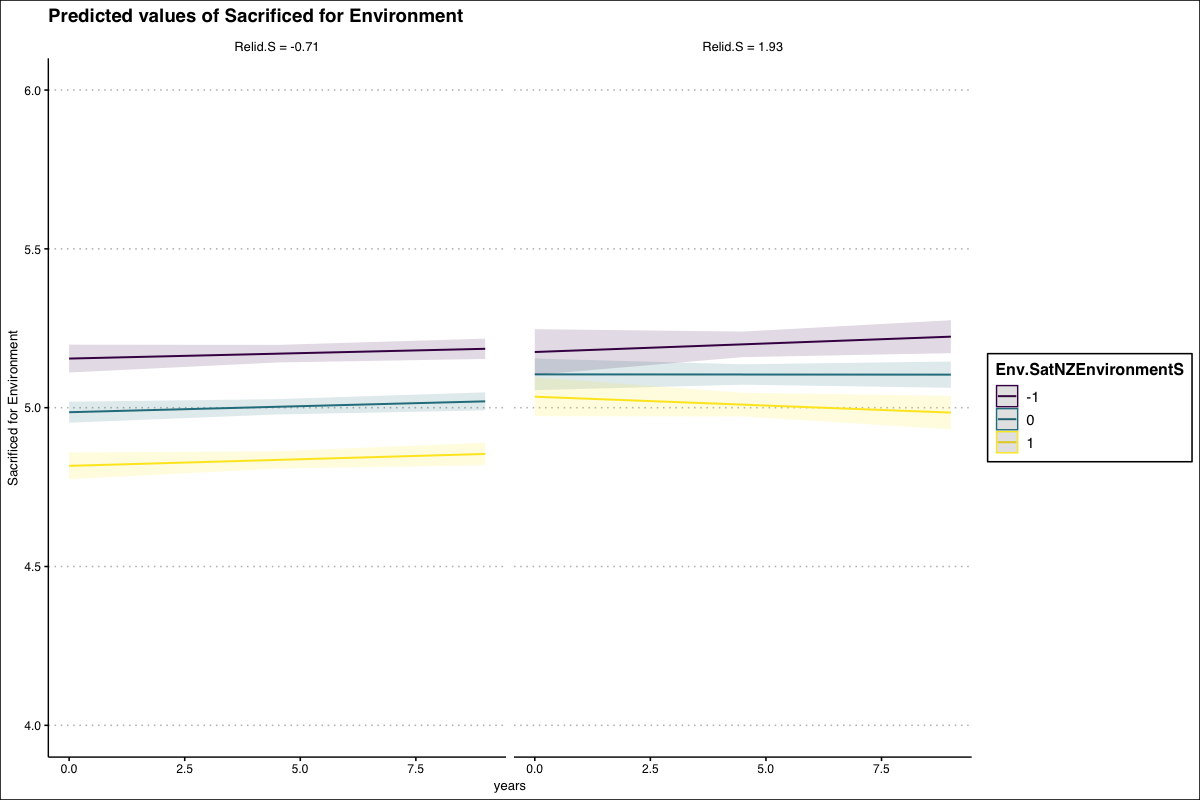
\includegraphics[width=.8\textwidth,height=\textheight,keepaspectratio]{Figures/X_SACRIFICEMADE_Env.SatNZEnvironmentS_Relid.S.png}
%\caption{}
\end{figure}
\end{frame}

\begin{frame}{What what predicts pro-environmental priorities?}

\begin{alertblock}{Government spending on motorways}
"Increased government spending on new motorways."
\end{alertblock}

\begin{alertblock}{Government spending on public transport}
"Government subsidy of public transport."
\end{alertblock}

\begin{alertblock}{Protection of New Zealand Native Species}
"Protecting New Zealand’s native species should be a national priority."
\end{alertblock}

    
\end{frame}

\begin{frame}{(dis)Satisfaction with the NZ environment predicts lower support for Motorway Spending (a revealed CO$_2$ preference).}
\begin{figure}
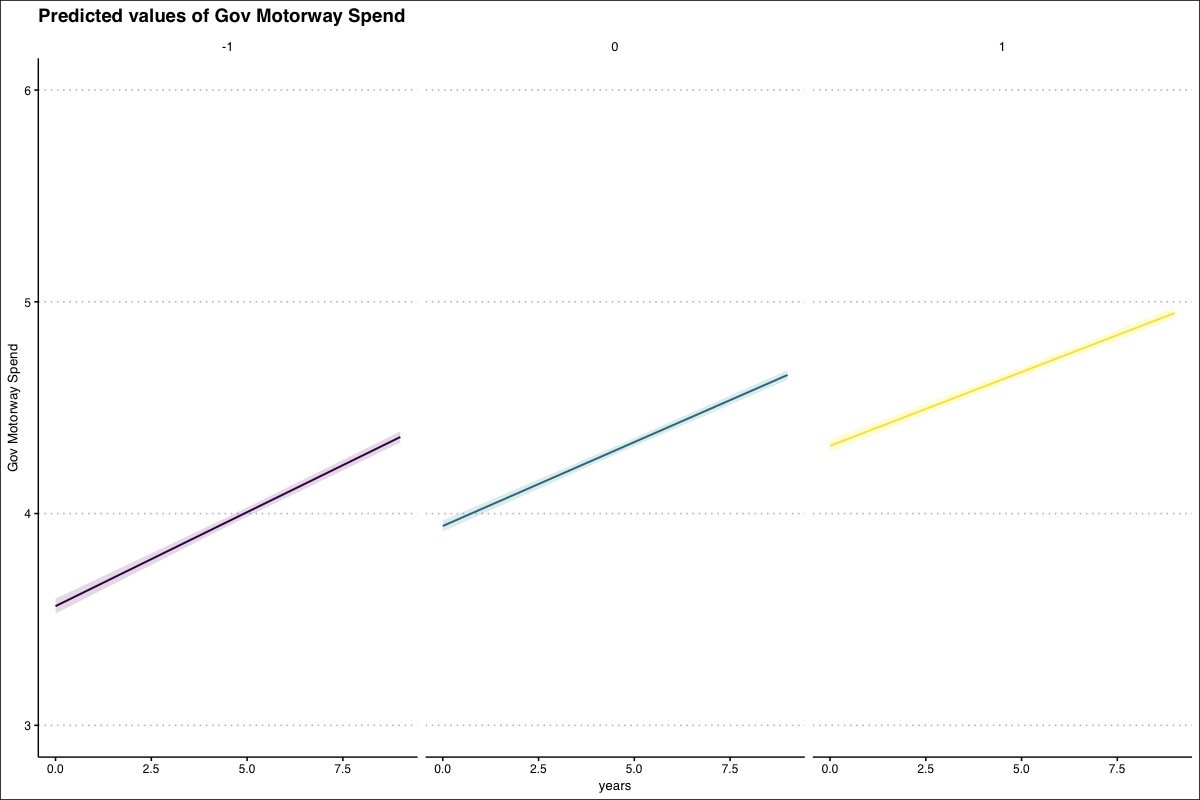
\includegraphics[width=.8\textwidth,height=\textheight,keepaspectratio]{Figures/XY_PLOT_Env.MotorwaySpend.SATENVIRON.png}
%\caption{}
\end{figure}
\end{frame}

\begin{frame}{(dis)Satisfaction with the NZ environment predicts greater support for public transport spending (a revealed CO$_2$ preference).}
\begin{figure}
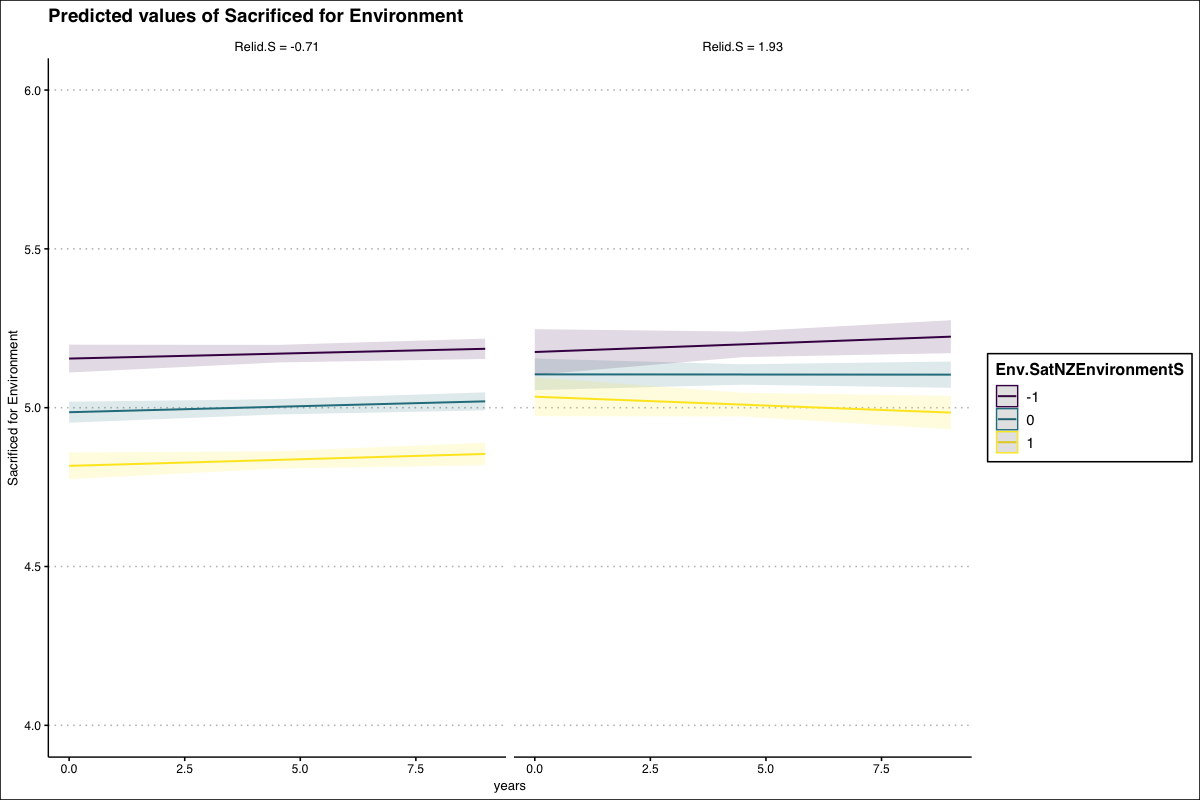
\includegraphics[width=.8\textwidth,height=\textheight,keepaspectratio]{Figures/X_SACRIFICEMADE_Env.SatNZEnvironmentS_Relid.S}
%\caption{}
\end{figure}
\end{frame}

\begin{frame}{(dis)Satisfaction with the NZ environment predicts greater support for protection of NZ species.}
\begin{figure}
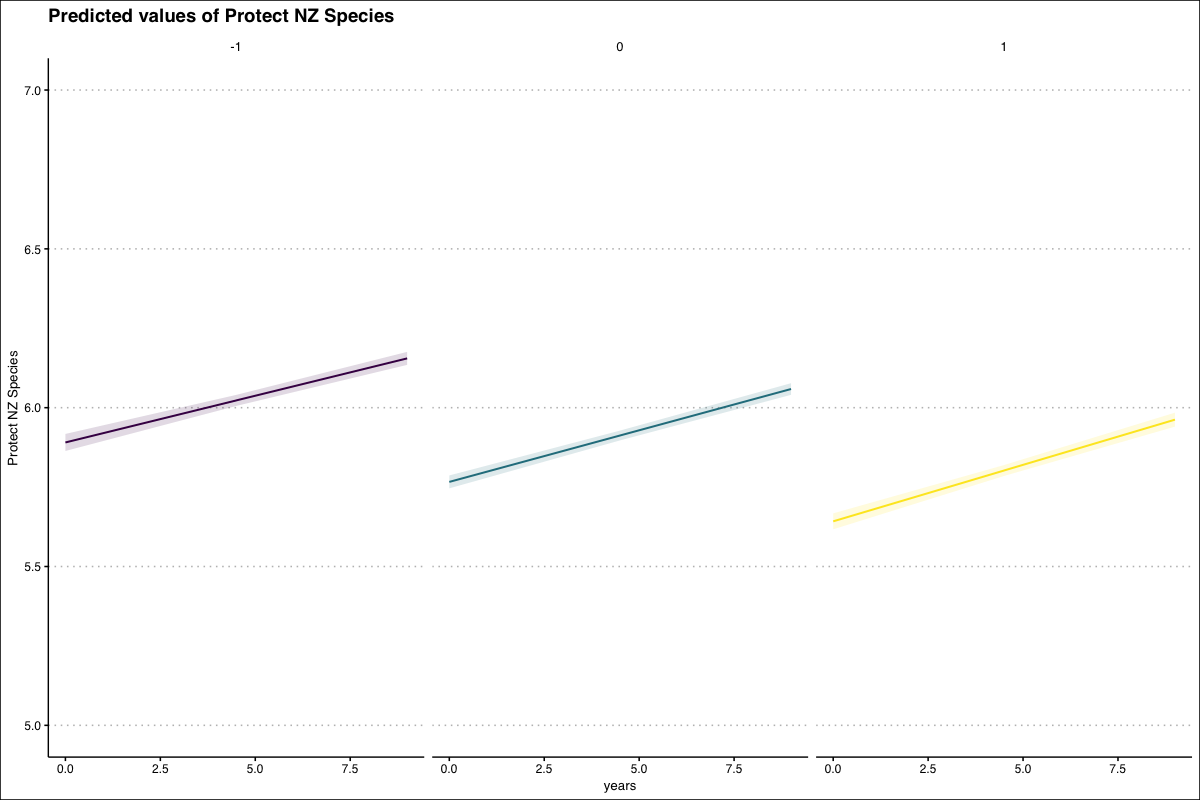
\includegraphics[width=.8\textwidth,height=\textheight,keepaspectratio]{Figures/XY_PLOT_Env.NATIVE.SPECIES.SATENVIRON.png}
%\caption{}
\end{figure}
\end{frame}


\section{Summary}

\begin{frame}{Take Homes}

  % Keep the summary *very short*.
  \begin{itemize}
  \item
         The \alert{first message}: compared with a decade ago, New Zealanders are substantially {\bf more (1) aware} and {\bf (2) more concerned about climate change}.
        \pause
  \item
    The  \alert{second message}: {\bf sacrifice} for the environment {\bf has been slow to follow} this awareness.
    \pause
    
    \item
    The  \alert{third message}: {\bf education is increasingly important} for climate awareness and behaviours.
    \pause
    
     \item
    The  \alert{fourth message}: recruit religious people: though less concerned about climate,{\bf religious people are more likely to believe they can make a difference} to the environment and {\bf more likely to sacrifice} for the environment.
     \pause
     
    \item
    The  \alert{fifth message}: {\bf foster frustration over fear} to promote pro-environmental behavior and policies.
    
    \pause
    
  \end{itemize}

\end{frame}

\begin{frame}{Frustration >  Fear}

\begin{columns}
\column{0.55\textwidth}
\begin{figure}
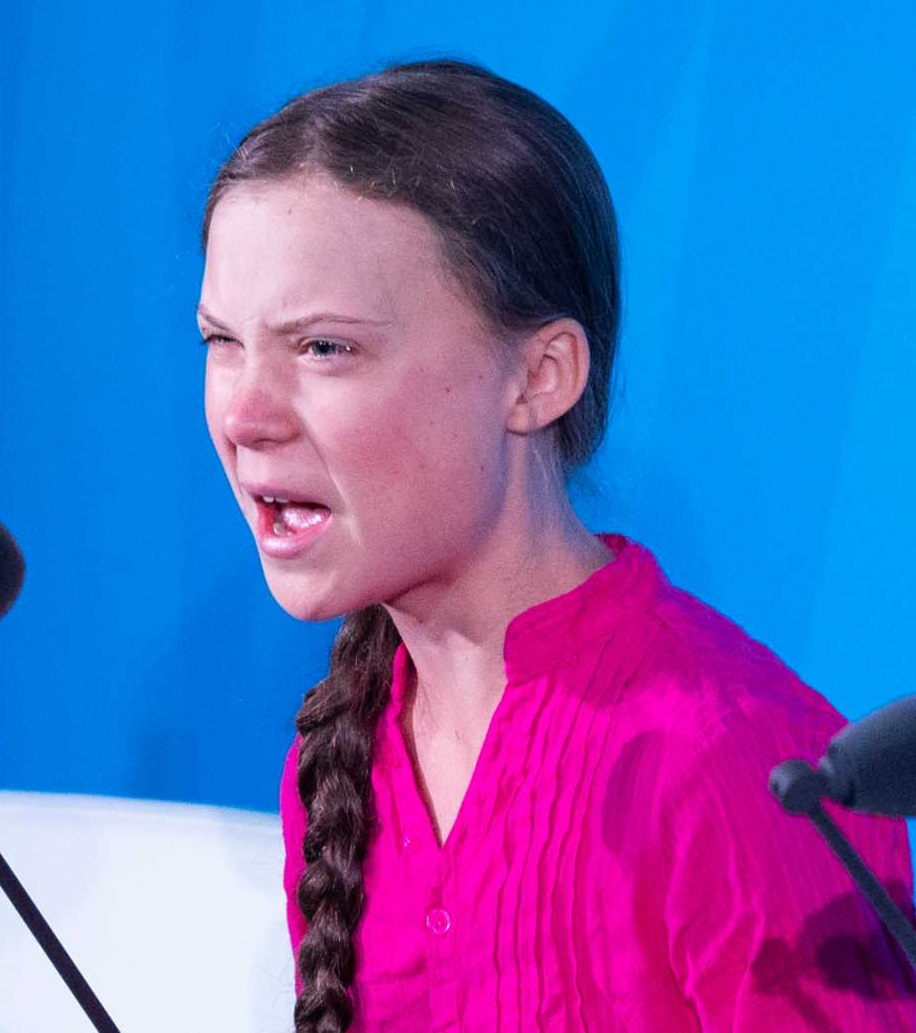
\includegraphics[width=1.02\textwidth,height=1.02\textheight,keepaspectratio]{Figures/Greta.jpg}
%\caption{}
\end{figure}


\column{0.45\textwidth}
\begin{figure}
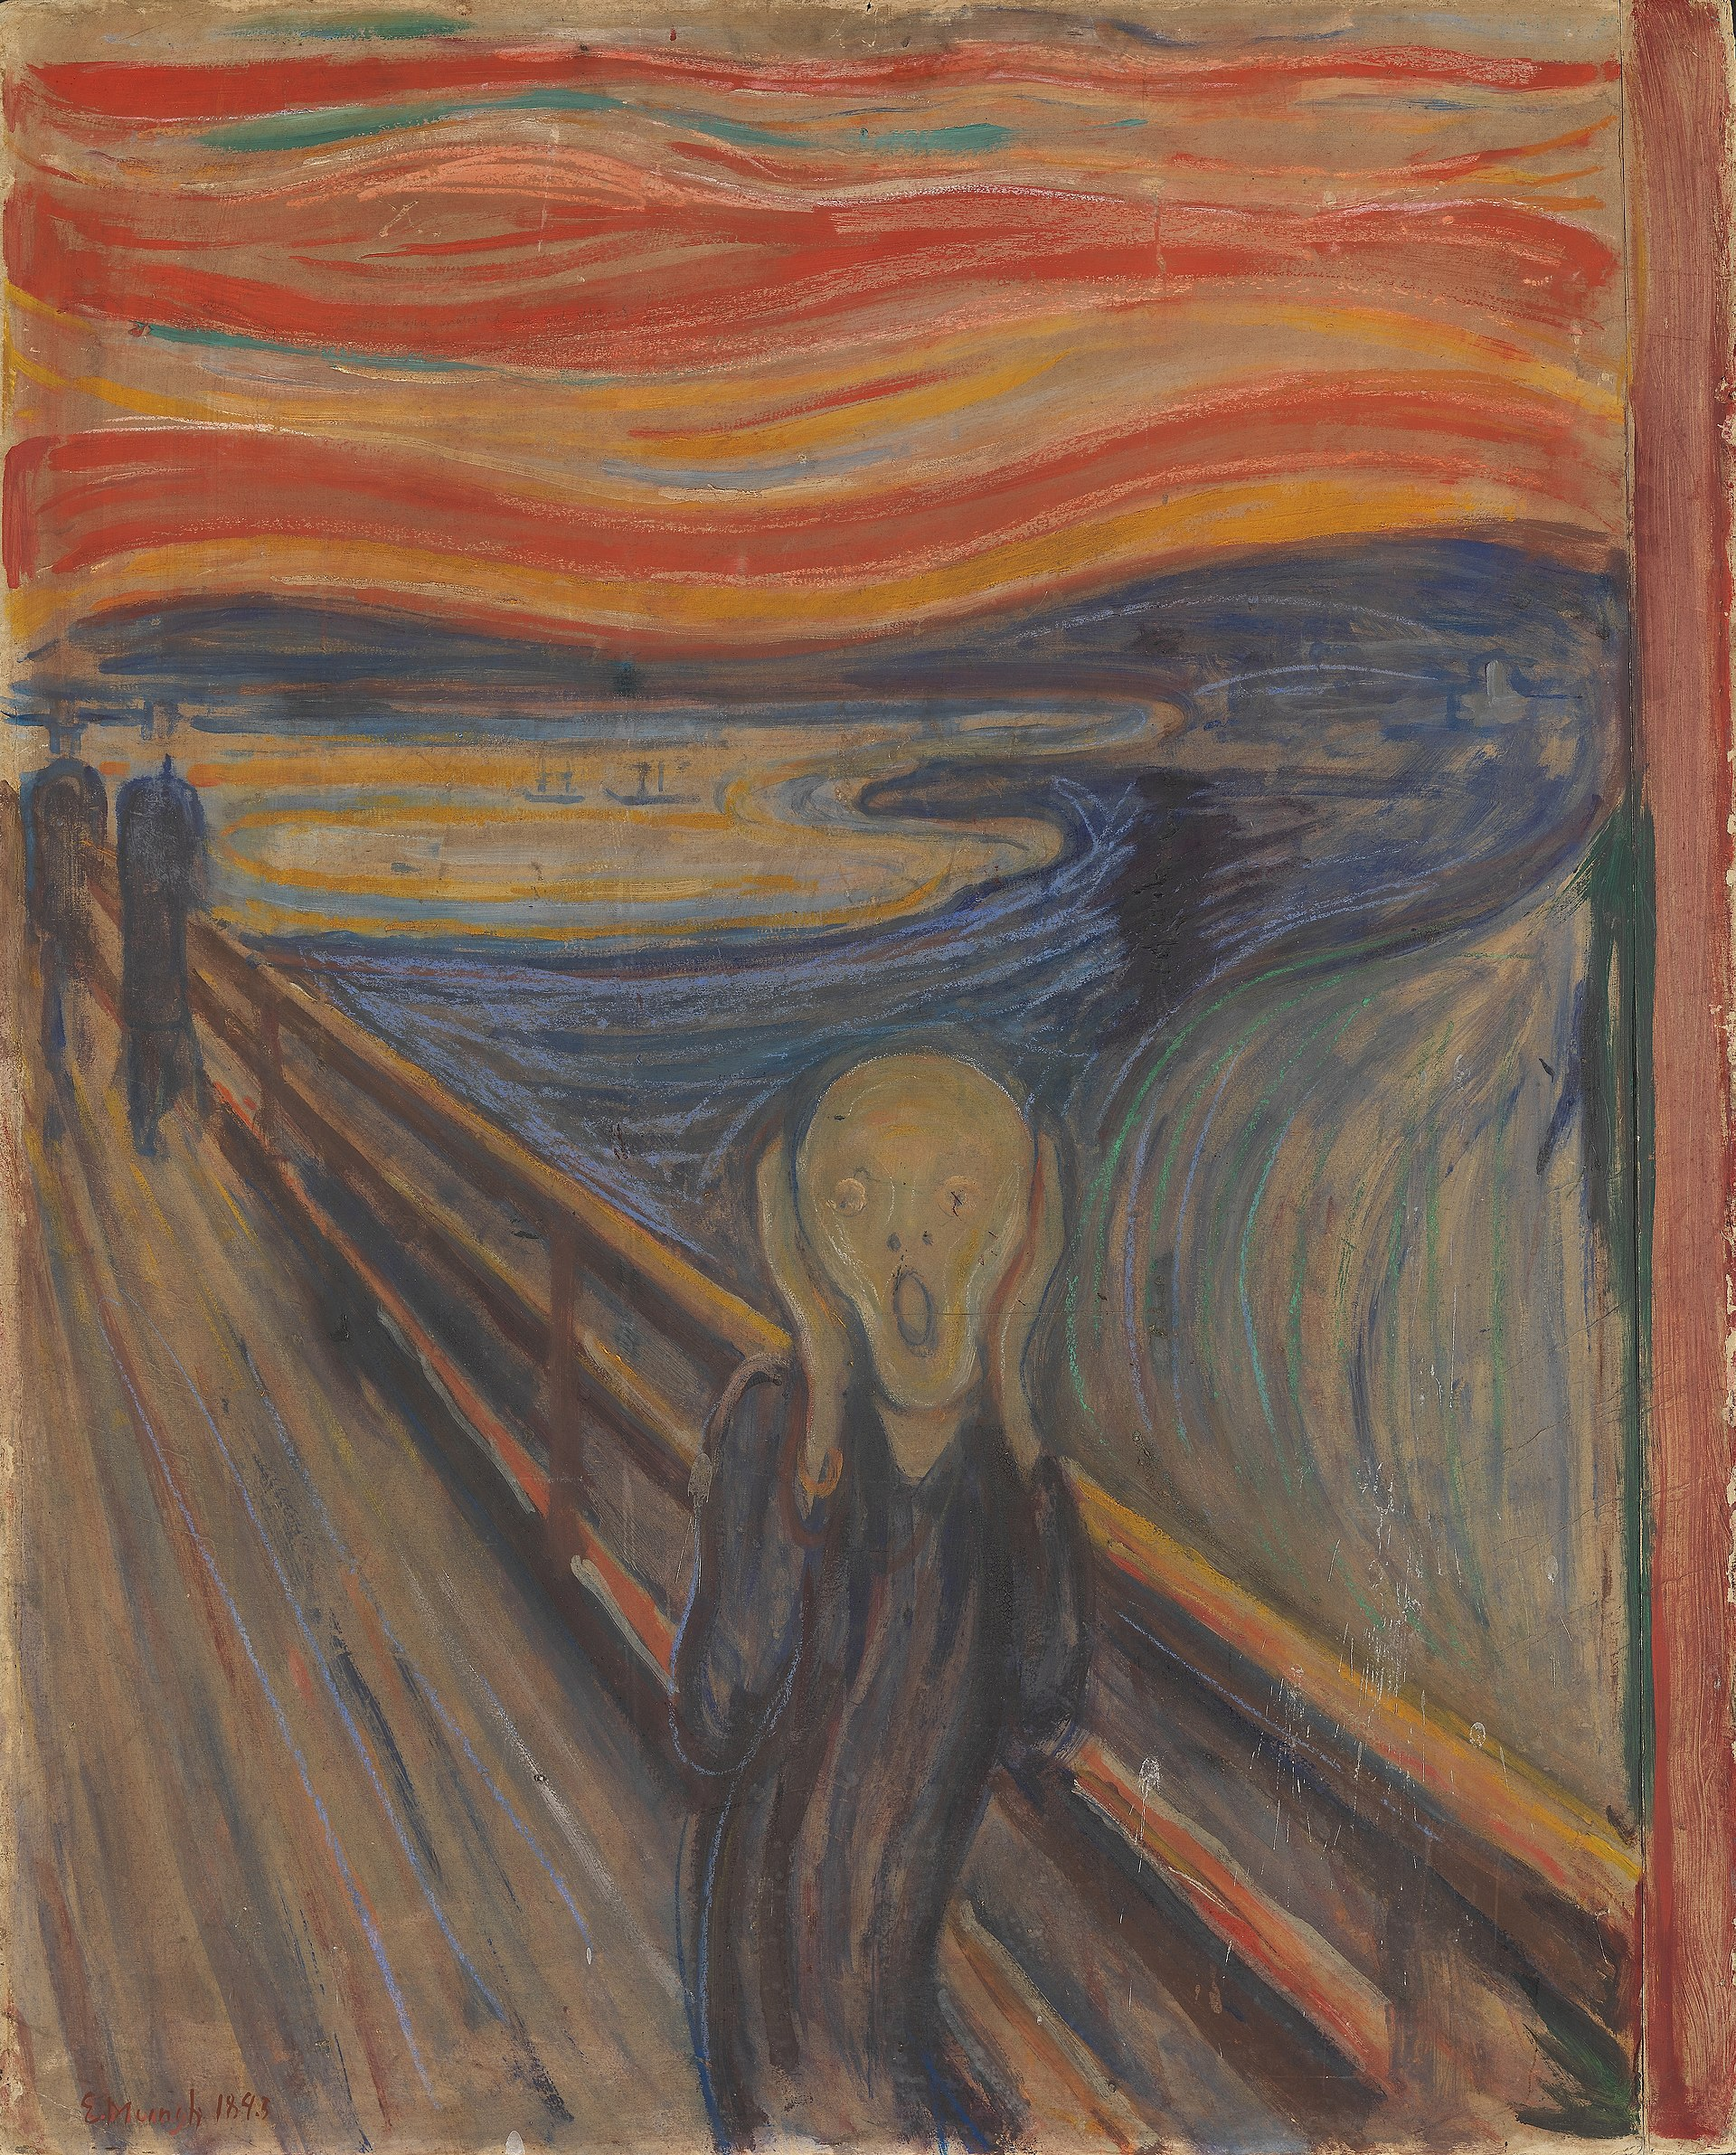
\includegraphics[width=1.05\textwidth,height=1.05\textheight,keepaspectratio]{Figures/Munchjpg.jpg}
%\caption{}
\end{figure}
\end{columns}
\end{frame}

% \begin{frame}{Thanks!}
% \begin{figure}
% 
\includegraphics[width=.99\textwidth,height=\textheight,keepaspectratio]{TRT_LOGO.png}
% %\caption{}
% \end{figure}
% \end{frame}


\begin{frame}
\frametitle{Thanks!}

\begin{columns}

\column{0.4\textwidth}
\begin{itemize}
\item Prof Dominic Johnson (University of Oxford) for the idea.
\item Prof Chris G. Sibley (University of Auckland) for the heavy lifting.
\item $>$ 50 NZAVS collaborators (join us!)
\item $>$ 61,535 New Zealanders who have participated for their time.
\item Templeton Religion Trust for their financial support.
\end{itemize}

\column{0.6\textwidth}
\centering
\begin{figure}

\includegraphics[width=\textwidth,height=\textheight,keepaspectratio]{TRT_LOGO.png}
%\caption{For their generous support}
\end{figure}
\end{columns}
\end{frame}


\begin{frame}{Cheers}
\centering
\texttt{joseph.bulbulia@vuw.ac.nz}
\end{frame}


%\section{Extra Slides}


\begin{frame}{Extra Slides: 2009-2018 Sample Demographic Indicators}
\begin{table}
\centering 
%\caption{Demographic Indicators}\label{}
\scalebox{.4}{
\begin{tabular}{ l c c c c c c c c c c }
\toprule
 &   \multicolumn{ 10 }{c}{ Wave }\\ 
  & 2009 & 2010 & 2011 & 2012 & 2013 & 2014 & 2015 & 2016 & 2017 & 2018 \\ 
 & n = 5523 & n = 4430 & n = 6652 & n = 11300 & n = 17241 & n = 15801 & n = 13929 & n = 20402 & n = 17017 & n = 18020 \\ 
 \midrule
Age &   &   &   &   &   &   &   &   &   &  \\ 
\hspace{6pt}   & 48.7 (15.3) & 51.0 (15.2) & 50.7 (15.8) & 49.7 (14.9) & 48.1 (14.0) & 49.3 (14.0) & 50.8 (13.9) & 50.2 (13.8) & 51.3 (13.8) & 52.3 (13.6)\\ 
EthnicCats &   &   &   &   &   &   &   &   &   &  \\ 
\hspace{6pt}    Euro & 4050 (73.3\%) & 3341 (75.4\%) & 4650 (69.9\%) & 8375 (74.1\%) & 13166 (76.4\%) & 12573 (79.6\%) & 11113 (79.8\%) & 16363 (80.2\%) & 13844 (81.4\%) & 14622 (81.1\%)\\ 
\hspace{6pt}    Maori & 890 (16.1\%) & 687 (15.5\%) & 721 (10.8\%) & 1743 (15.4\%) & 2168 (12.6\%) & 1973 (12.5\%) & 1668 (12\%) & 2244 (11\%) & 2002 (11.8\%) & 2081 (11.5\%)\\ 
\hspace{6pt}    Pacific & 206 (3.7\%) & 139 (3.1\%) & 140 (2.1\%) & 408 (3.6\%) & 471 (2.7\%) & 433 (2.7\%) & 351 (2.5\%) & 449 (2.2\%) & 319 (1.9\%) & 335 (1.9\%)\\ 
\hspace{6pt}    Asian & 227 (4.1\%) & 164 (3.7\%) & 219 (3.3\%) & 478 (4.2\%) & 679 (3.9\%) & 632 (4\%) & 492 (3.5\%) & 806 (4\%) & 646 (3.8\%) & 678 (3.8\%)\\ 
\hspace{6pt}    \emph{missing} & 150 (2.7\%) & 99 (2.2\%) & 922 (13.9\%) & 296 (2.6\%) & 757 (4.4\%) & 190 (1.2\%) & 305 (2.2\%) & 540 (2.6\%) & 206 (1.2\%) & 304 (1.7\%)\\ 
Edu &   &   &   &   &   &   &   &   &   &  \\ 
\hspace{6pt}   & 5.1 (2.8) & NaN (\emph{missing}) & NaN (\emph{missing}) & 5.7 (2.8) & 5.9 (2.8) & 6.1 (2.8) & 6.2 (2.8) & 6.3 (2.7) & 6.5 (2.7) & 6.5 (2.7)\\ 
Male &   &   &   &   &   &   &   &   &   &  \\ 
\hspace{6pt}    0 & 3338 (60.4\%) & 2729 (61.6\%) & 4161 (62.6\%) & 7085 (62.7\%) & 10890 (63.2\%) & 9966 (63.1\%) & 8707 (62.5\%) & 12806 (62.8\%) & 10756 (63.2\%) & 11287 (62.6\%)\\ 
\hspace{6pt}    1 & 2185 (39.6\%) & 1701 (38.4\%) & 2491 (37.4\%) & 4215 (37.3\%) & 6351 (36.8\%) & 5782 (36.6\%) & 5172 (37.1\%) & 7528 (36.9\%) & 6203 (36.5\%) & 6690 (37.1\%)\\ 
\hspace{6pt}    \emph{missing} & 0 (0\%) & 0 (0\%) & 0 (0\%) & 0 (0\%) & 0 (0\%) & 53 (0.3\%) & 50 (0.4\%) & 68 (0.3\%) & 58 (0.3\%) & 43 (0.2\%)\\ 
NZdep &   &   &   &   &   &   &   &   &   &  \\ 
\hspace{6pt}   & 5.0 (2.8) & 4.9 (2.8) & 4.6 (2.7) & 4.9 (2.8) & 4.8 (2.8) & 4.7 (2.8) & 4.7 (2.8) & 4.6 (2.7) & 4.6 (2.7) & 4.6 (2.7)\\ 
Pol Orient &   &   &   &   &   &   &   &   &   &  \\ 
\hspace{6pt}   & 3.8 (1.2) & 4.0 (1.3) & 3.7 (1.4) & 3.7 (1.3) & 3.6 (1.3) & 3.6 (1.3) & 3.6 (1.3) & 3.6 (1.4) & 3.6 (1.4) & 3.6 (1.4)\\ 
Relid &   &   &   &   &   &   &   &   &   &  \\ 
\hspace{6pt}   & 2.3 (2.8) & 2.2 (2.8) & 1.9 (2.7) & 2.0 (2.7) & 1.9 (2.7) & 1.9 (2.7) & 2.0 (2.7) & 1.8 (2.6) & 1.7 (2.6) & 1.7 (2.6)\\ 
Urban &   &   &   &   &   &   &   &   &   &  \\ 
\hspace{6pt}    0 & 2220 (40.2\%) & 1785 (40.3\%) & 2161 (32.5\%) & 3815 (33.8\%) & 5583 (32.4\%) & 5158 (32.6\%) & 4621 (33.2\%) & 7039 (34.5\%) & 3089 (18.2\%) & 3220 (17.9\%)\\ 
\hspace{6pt}    1 & 3269 (59.2\%) & 2623 (59.2\%) & 4006 (60.2\%) & 7310 (64.7\%) & 11531 (66.9\%) & 10439 (66.1\%) & 8986 (64.5\%) & 13124 (64.3\%) & 13688 (80.4\%) & 14512 (80.5\%)\\ 
\hspace{6pt}    \emph{missing} & 34 (0.6\%) & 22 (0.5\%) & 485 (7.3\%) & 175 (1.5\%) & 127 (0.7\%) & 204 (1.3\%) & 322 (2.3\%) & 239 (1.2\%) & 240 (1.4\%) & 288 (1.6\%)\\ 
\bottomrule

\end{tabular}
}
\end{table}

\end{frame}


\begin{frame}{Coefficient Plot: Climate Change is Real}
\begin{figure}
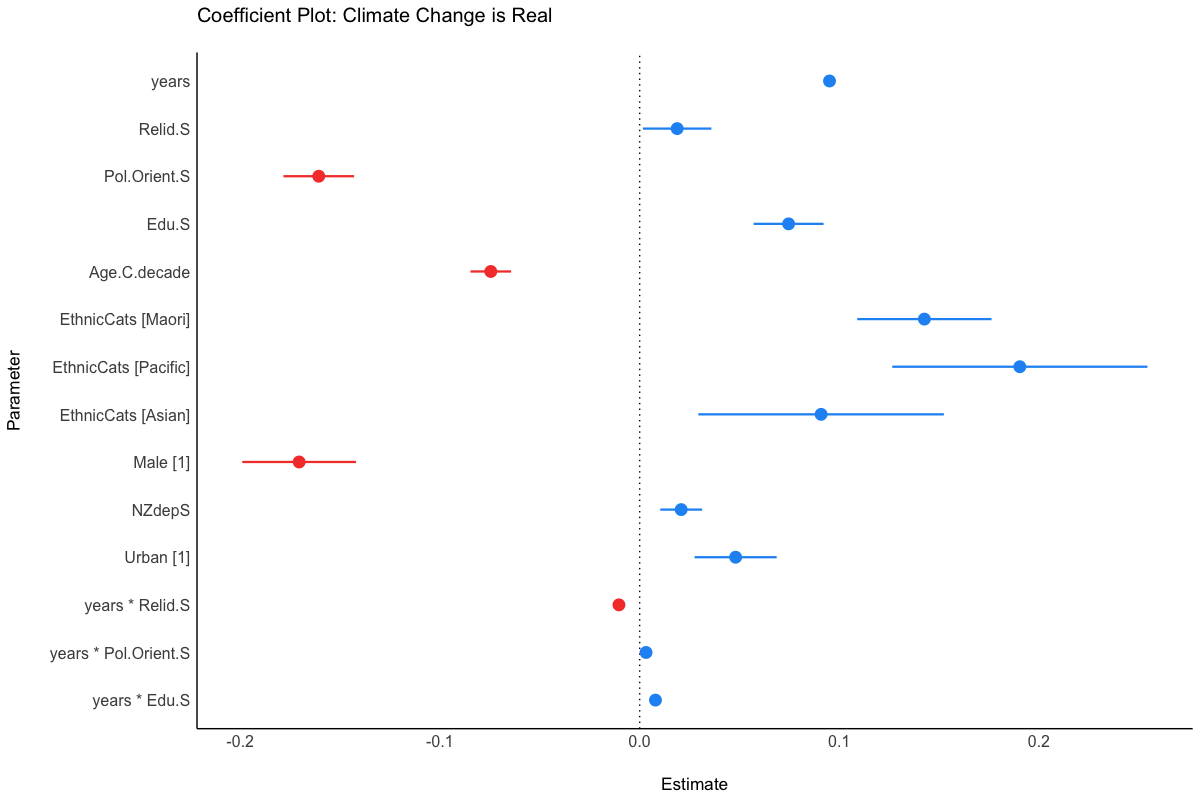
\includegraphics[width=.99\textwidth,height=\textheight,keepaspectratio]{Figures/mREAL.png}
%\caption{}
\end{figure}
\end{frame}

\begin{frame}{Coefficient Plot: Environmental Concern}
\begin{figure}
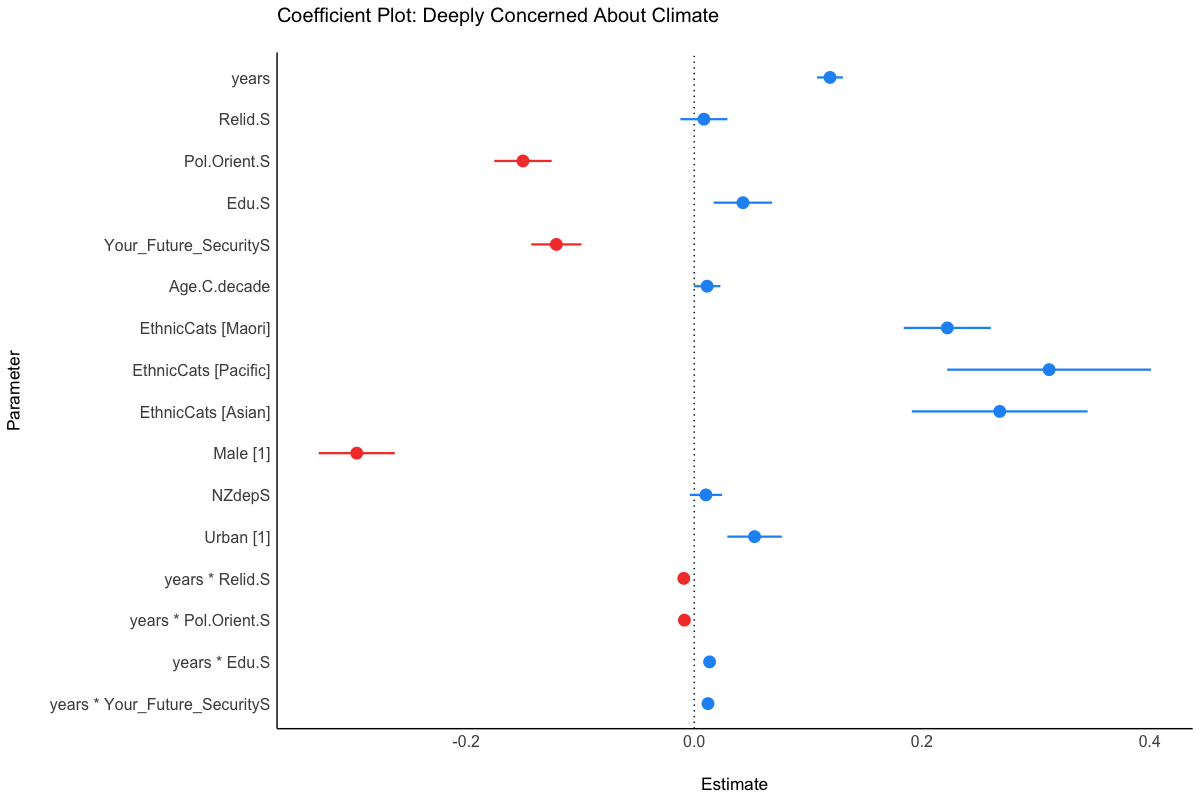
\includegraphics[width=.99\textwidth,height=\textheight,keepaspectratio]{Figures/mCONCERN.png}
%\caption{}
\end{figure}
\end{frame}


\begin{frame}{Coefficient Plot: Environmental Efficacy}
\begin{figure}
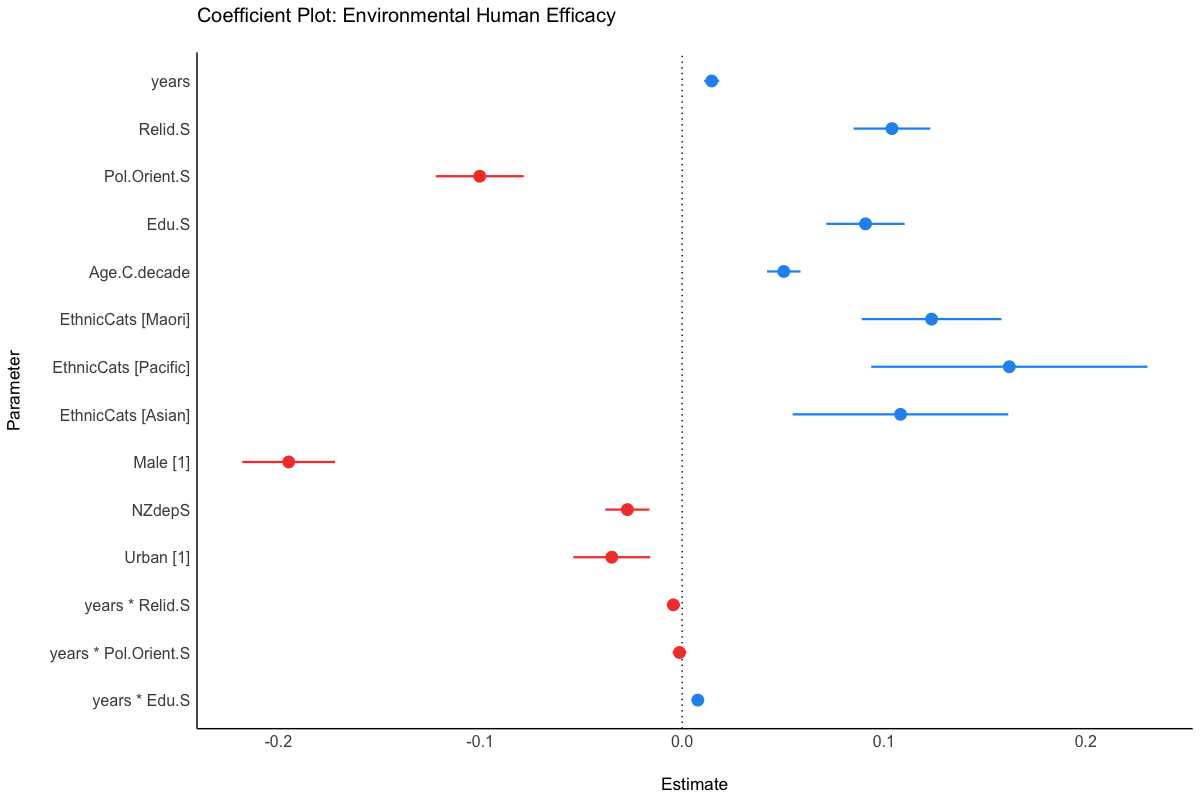
\includegraphics[width=.99\textwidth,height=\textheight,keepaspectratio]{Figures/mEFFICACY.png}
%\caption{}
\end{figure}
\end{frame}

\begin{frame}{Coefficient Plot: Sacrifice Made}
\begin{figure}
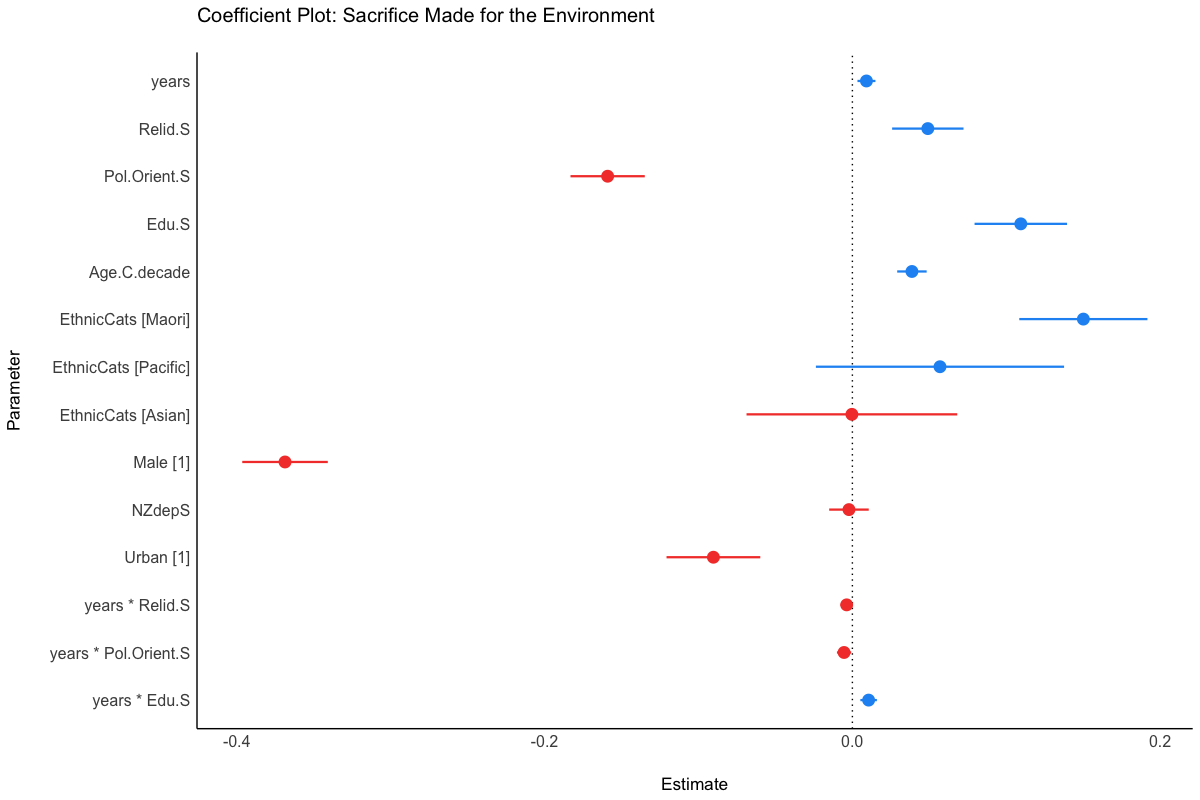
\includegraphics[width=.99\textwidth,height=\textheight,keepaspectratio]{Figures/mSACRIFICEMADE.png}
%\caption{}
\end{figure}
\end{frame}

\end{document}